%; whizzy subsection   
\documentclass[a4paper,english,french]{article}

\usepackage[utf8]{inputenc}

\usepackage{amsmath}
\usepackage{amsfonts}
\usepackage[T1]{fontenc}
\usepackage{lmodern}
\usepackage{babel}
\usepackage{graphicx}
\usepackage{leftidx}
\usepackage{mathabx}
\usepackage{mathrsfs}
\usepackage[version=3]{mhchem}
\usepackage{variations}
\usepackage[np]{numprint}

\usepackage{hyperref}

\hypersetup{pdftitle={Fonctionnement : derrière les coulisses,
    description des programmes}, pdfauthor={Lionel Guez},
  pdfborderstyle={/S/U/W 1}}

\newcommand{\ud}{\mathrm{d}}
\newcommand{\uD}{\mathrm{D}}
\newcommand{\Eng}[1]{\textit{\foreignlanguage{english}{#1}}}

\DeclareMathOperator{\tgh}{th}
\DeclareMathOperator{\Arcsin}{Arcsin}
\DeclareMathOperator{\sgn}{sgn}
\DeclareMathOperator{\sinc}{sinc}

\graphicspath{{Graphiques/}}

\author{Lionel GUEZ}

\title{Manuel pour LMDZE -- Fonctionnement : derrière les coulisses,
  description des programmes}

\begin{document}

\maketitle
\tableofcontents
\listoffigures

\section{Divers}

LMDZE dérive à peu près (à quelques mélanges près) de la révision 691
de LMDZ (avril 2006).

Il n'y a aucune directive include dans le programme. Tous les fichiers
Fortran ont le suffixe \verb+.f90+ et sont au format libre.
\begin{verbatim}
ack -f | wc -l
\end{verbatim}
donne environ \np{4e2} fichiers.
\begin{verbatim}
ack --fortran -f | wc -l
\end{verbatim}
donne environ \np{3e2} fichiers.
\begin{verbatim}
ack -f --print0 | wc -l --files0-from=-
\end{verbatim}
donne environ \np{5e4} lignes.
\begin{verbatim}
ack --fortran -f --print0 | wc -l --files0-from=-
\end{verbatim}
donne environ \np{4e4} lignes.

Le programme est divisé en une partie ``dynamique'' et une partie
``physique''. La dynamique est vraiment à trois dimensions.  La
physique est essentiellement unidimensionnelle, sur la verticale : il
y a très peu d'interactions horizontales dans la partie ``physique''.
Lignes directrices de la conception du programme :
\begin{itemize}
\item Séparation entre dynamique et physique.
\item La dynamique ne contient aucune référence au contenu des
  paramétrisations physiques, aucune spécificité terrestre, pour
  pouvoir être associée à différentes physiques, sur différentes
  planètes.
\item La physique ne fait aucune hypothèse sur le maillage horizontal,
  elle traite simplement un ensemble de positions horizontales qui
  pourraient être quelconques à la surface de la Terre, et en nombre
  quelconque (en particulier un nombre réduit à 1). Ainsi, la physique
  peut être associée à différentes dynamiques, par exemple sur une
  grille icosaédrique.
\end{itemize}

Au plus haut niveau, parties du programme \verb+gcm+ : calcul des
tendances (\verb+caldyn+), intégration (\verb+integrd+), physique,
dissipation (\verb+dissip+), advection. Variables principales de la
dynamique : vent covariant (\verb+ucov+, \verb+vcov+), température
potentielle, pression à la surface. La vitesse verticale $\omega$ se
déduit par quelque chose comme une relation de fermeture. Variables
principales de la physique : vent naturel, température naturelle. Dans
la physique, il n'y a pas d'échange horizontal entre les mailles. Un
problème fondamental est l'utilisation d'une grille rectangulaire en
latitudes et longitudes pour couvrir la sphère. Les mailles de la
grille n'ont pas la même surface.  La solution choisie pour résoudre
ce problème est le filtrage. Le filtre est très coûteux : il faut
connaître le champ en entier pour le calculer en un point
particulier. Par ailleurs, le programme calcule à de nombreuses
occasions des valeurs moyennes aux pôles, à partir des mailles
pôlaires (à chaque pôle, autant de mailles pôlaires que de longitudes
dans la grille).

La variable omega en argument de la procédure physiq n'est pas
$\frac{\uD p}{\uD t}$. C'est peut-être plutôt
$(\partial_s p) \frac{\uD s}{\uD t}$, où $s$ est la coordonnée verticale
hybride sigma-pression.

Le répertoire \verb+phylmd+ contient ce qui concerne la 
physique. Le répertoire \verb+dyn3d+ contient ce qui concerne 
la dynamique.

\verb+histins.nc+ contient des instantanés. \verb+ini_histins+
initialise le fichier \verb+histins.nc+, ce qui inclut
l'initialisation de variables avec le sous-programme \verb+histdef+.
L'écriture du contenu d'une variable se fait avec le sous-programme
\verb+histwrite_phy+.

Dans la procédure guide, la variable tau vaut, en notation
mathématique :
\begin{equation*}
  \frac{4\ \mathrm{itau}}{\mathrm{day\_step}}
  - E\left(\frac{4\ \mathrm{itau}}{\mathrm{day\_step}} \right)
\end{equation*}
\`A quelle période correspond l'incrément de guidage ? Considérons par
exemple le guidage sur le vent et prenons l'origine des temps au début
de la simulation. Soit une valeur de itau multiple de iperiod. \`A
l'itération itau de leapfrog, on a le vent définitif à la date itau *
dtvr. On commence cette itération en appliquant le guidage. Le champ
vers lequel on rappelle est le champ interpolé à la date itau *
dtvr. On applique un incrément de guidage correspondant au rappel vers
ce champ pendant iperiod * dtvr. On peut remarquer que cet incrément
est appliqué à l'iération 0, et qu'il est appliqué pour la dernière
fois à l'itération itaufin - iperiod. Les seuls états qui ont un sens
sont ceux qui ont reçu toutes les tendances (avec leurs différents pas
de temps), y compris la tendance physique. Il faut donc considérer que
l'incrément de guidage est appliqué par avance. C'est-à-dire que
l'incrément appliqué à l'itération itau correspond au guidage sur la
période qui va de itau * dtvr à (itau + iperiod) * dtvr. Et le rappel
se fait vers le champ interpolé au début de la période de guidage.

Le fichier de guidage doit commencer par un état à t = 0 et aller au
moins jusqu'à la date itaufin * dtvr. Même si le champ vers lequel on
rappelle ne sera jamais l'état à la date itaufin * dtvr (puisque le
dernier guidage est à itaufin - iperiod), l'état à la date itaufin *
dtvr est bien utilisé pour interpoler les champs de rappel dans les
derniers guidage.

Cf. figure (\ref{fig:temperature}).
\begin{figure}
  \centering
  \includegraphics{temperature}
  \caption[Température dans physiq]{Variables contenant une
    température dans la procédure physiq, verticalement réparties
    selon leur signification.}
  \label{fig:temperature}
\end{figure}
Modifications de la variable \verb+t_seri+ dans la procédure
\verb+physiq+ :
\begin{itemize}
\item évaporation
\item \verb+d_t_vdf+
\item \verb+d_t_con+
\item \verb+d_t_ajs+ ou \verb+calltherm+
\item \verb+d_t_lsc+
\item \verb+heat - cool+
\item \verb+d_t_oro+
\item \verb+d_t_lif+
\item \verb+d_t_ec+
\end{itemize}

Cf. figure (\ref{fig:ps_gcm}).
\begin{figure}
  \centering
  \includegraphics{ps_gcm}
  \caption[Flot de la pression à la surface dans gcm]{Flot de la
    variable pression à la surface dans le programme gcm.}
  \label{fig:ps_gcm}
\end{figure}
La variable masse dans la procédure leapfrog n'est modifiée que par
caldyn et integrd.

Dans LMDZ, pour permettre un zoom, le système de coordonnées
curvilignes est $(x, y, s)$ où $x = x(\lambda)$, $y = y(\phi)$ et $s$
est la coordonnée verticale hybride $\sigma$-pression. Cf. la
note
\href{../../../Documentation_LMDZ/Dynamics_texfol/dynamics.pdf}{Discrétisation
  des équations de la dynamique dans le modèle LMDZ} (équations
(1)). La base naturelle associée est :
\begin{align*}
  & \mathbf{e}_x
    = (\partial_\lambda \mathbf{r})_{\phi, s} \frac{\ud \lambda}{\ud x} \\
  & \mathbf{e}_y
    = (\partial_\phi \mathbf{r})_{\lambda, s} \frac{\ud \phi}{\ud y} \\
  & \mathbf{e}_s = (\partial_s \mathbf{r})_{\lambda, \phi} 
\end{align*}
D'où,
d'après \href{../Vertical_grid_texfol/vertical_grid.pdf}{Maillage
  vertical} :
\begin{align*}
  & \mathbf{e}_x
    = \frac{\ud \lambda}{\ud x}
    \left[
    \mathscr{R} \mathbf{i}
    +
    \left(
    (\partial_\lambda z)_p - \frac{b}{\rho g} \partial_\lambda p_s
    \right)
    \mathbf{k}
    \right] \\
  & \mathbf{e}_y
    =  \frac{\ud \phi}{\ud y}
    \left[
    r \mathbf{j}
    +
    \left(
    (\partial_\phi z)_p - \frac{b}{\rho g} \partial_\phi p_s
    \right)
    \mathbf{k}
    \right] \\
  & \mathbf{e}_s
    = - \frac{1}{\rho g}
    \left(\frac{\ud a}{\ud s} + p_s \frac{\ud b}{\ud s} \right) \mathbf{k}
\end{align*}
D'où les composantes contravariantes du vent :
\begin{align*}
  & V^x = \frac{u}{\mathscr{R}} \frac{\ud x}{\ud \lambda} \\
  & V^y = \frac{v}{r} \frac{\ud y}{\ud \phi}
\end{align*}
La base duale est :
\begin{align*}
  & \mathbf{e}^x = \frac{\ud x}{\ud \lambda} \nabla \lambda \\
  & \mathbf{e}^y = \frac{\ud y}{\ud \phi} \nabla \phi \\
  & \mathbf{e}^s = \nabla s
\end{align*}
D'où,
d'après \href{../Vertical_grid_texfol/vertical_grid.pdf}{Maillage
  vertical} :
\begin{align*}
  & \mathbf{e}^x = \frac{1}{\mathscr{R}} \frac{\ud x}{\ud \lambda} \mathbf{i} \\
  & \mathbf{e}^y = \frac{1}{r} \frac{\ud y}{\ud \phi} \mathbf{j} \\
  & \mathbf{e}^s
    = \frac{1}{\frac{\ud a}{\ud s} + p_s \frac{\ud b}{\ud s}}
  [\rho (\nabla \Phi)_p - \rho g \mathbf{k} - b \nabla p_s]
\end{align*}
D'où les composantes covariantes du vent :
\begin{align*}
  & V_x = \mathscr{R} u \frac{\ud \lambda}{\ud x} \\
  & V_y = r v \frac{\ud \phi}{\ud y}
\end{align*}
Les tableaux \verb+cu_2d+ et \verb+cv_2d+ sont écrits dans
\verb+restart.nc+. Pour un maillage sans zoom :
\begin{align*}
  & c_u = a \cos \phi\ \delta \lambda = a (\cos \phi) \frac{2
    \pi}{\mathtt{iim}} \\
  & c_v = a \delta \phi = a \frac{\pi}{\mathtt{jjm}}
\end{align*}

Procédure tourpot. On calcule la circulation du vent sur une cellule
horizontale. Pour que le résultat soit la surface de la maille
(positive) multipliée par la composante de la vorticité sur le vecteur
$\mathbf{k}$, il faut que le contour de la cellule soit orienté dans
le sens trigonométrique. Cf. figure (\ref{fig:tourpot}).
\begin{figure}
  \centering
  \includegraphics{tourpot}
  \caption[Vorticité dans tourpot]{Calcul de la vorticité dans
    tourpot. Le point bleu est celui où l'on calcule la vorticité. Le
    contour est celui d'une cellule horizontale du maillage, orienté
    dans le sens trigonométrique.}
  \label{fig:tourpot}
\end{figure}
La circulation est :
\begin{equation*}
  C = \oint \mathbf{V} \cdot \ud \mathbf{r}
\end{equation*}
Soit :
\begin{multline*}
  C = u\left(\lambda, \phi - \frac{\delta \phi}{2} \right) a
  \cos\left(\phi - \frac{\delta \phi}{2} \right) \delta \lambda
  + v\left(\lambda + \frac{\delta \lambda}{2}, \phi \right)
  a \delta \phi \\
  - u\left(\lambda, \phi + \frac{\delta \phi}{2} \right) a
  \cos\left(\phi + \frac{\delta \phi}{2} \right) \delta \lambda
  - v\left(\lambda - \frac{\delta \lambda}{2}, \phi \right)
  a \delta \phi
\end{multline*}
Soit, en notation discrète, en remarquant que les indices de latitude
varient en sens inverse des latitudes, en notant $\tilde u$ et $\tilde
v$ les composantes du vent covariant :
\begin{equation*}
  C = \tilde u_{i, j + \frac{1}{2}} + \tilde v_{i + \frac{1}{2}, j}
  - \tilde u_{i, j - \frac{1}{2}} - \tilde v_{i - \frac{1}{2}, j}
\end{equation*}

Cf. figures \ref{fig:thermcell} et \ref{fig:wa}.
\begin{figure}
  \centering
  \includegraphics{thermcell}
  \caption[Procédure thermcell]{Procédure thermcell.}
  \label{fig:thermcell}
\end{figure}
\begin{figure}
  \centering
  \includegraphics{wa}
  \caption[Indi\c cages dans thermcell]{Procédure thermcell. Indi\c
    cages : l'ascendance provenant du niveau k traverse l'interface l
    avec une vitesse wa(k, l).}
  \label{fig:wa}
\end{figure}

\verb+grille_m+.
\begin{verbatim}
           (c)
        ----d-----
        | . . . .|
        |        |
     (b)a . * . .b(a)
        |        |
        | . . . .|
        ----c-----
           (d)
\end{verbatim}

ajsec remplace la température potentielle par sa moyenne sur la couche
statiquement instable. Cette moyenne est pondérée par la masse et la
fonction d’Exner. Il fait la même chose pour $q$. Cette pondération est
ce qu’il faut faire pour conserver l’énergie car enthalpie = Exner
$\times \theta$. Mais ça ne va pas conserver $q$, il faudrait pondérer
seulement par la masse.

Dans la procédure groupeun, jd peut valoir 0 ou 1. Pour une valeur
donnée de l, on peut montrer qu'au début de l'itération sur ig, j2
vaut \verb+2**ig+ et j1 vaut \verb|2**(ig - 1)+1|. Comme il y a un
accès à \verb+aire_2d(i, j)+ avec j valant \verb+j2-jd+, il faut que :
\begin{verbatim}
j2 - jd <= jjm + 1
\end{verbatim}
En particulier, pour jd valant 0 :
\begin{verbatim}
j2 <= jjm + 1
\end{verbatim}
C'est-à-dire :
\begin{verbatim}
2**ig <= jjm + 1
\end{verbatim}
Il faut donc :
\begin{verbatim}
2**ngroup <= jjm + 1
\end{verbatim}

\section{Rayonnement}

Le code de rayonnement est basé sur les algorithmes de Fouquart et
Bonnel (1980), a été écrit à l'ECMWF par Fouquart et J.-J. Morcrette,
a été repris dans Arpège et est resté figé dans Arpège dans l'état
dans lequel il était au cycle 15 (1996), a été adapté à partir de
cette version d'Arpège par Laurent Li pour LMDZ. Référence : Morcrette
(1990 k0997). Deux bandes dans le domaine ondes courtes, six bandes
dans le domaine ondes longues. Par rapport au code de 1990, le code de
LMDZ tient compte : des aérosols sulfatés pour la partie \Eng{clear
  sky shortwave} ; de \ce{CH4}, \ce{N2O}, des CFC pour la partie
\Eng{clear sky longwave}.

Calculs en amont du rayonnement : ozone, albédos diffus et direct pour
le shortwave, propriétés optiques des nuages (épaisseur optique,
émissivité). Concentrations de gaz à effet de serre définies en dehors
du code de rayonnement.

Le calcul du transfert radiatif (appel de radlwsw) n'est a priori pas
fait tous les pas de temps de la physique (ce qui est contrôlé par
\verb+nbapp_rad+) mais la variation de température due au rayonnement
est bien appliquée tous les pas de temps de la physique. Ce qui est
ajusté par le calcul de transfert radiatif, c'est donc la valeur de
l'incrément de température pour un pas de temps de la physique. Si le
calcul du transfert radiatif n'est pas fait tous les pas de temps de
la physique, quand on regarde la température à la surface à tous les
pas de temps de la physique, on voit des sauts au moment de l'appel du
transfert radiatif, pendant les heures de jour seulement. Ce qui
signifie que ces sauts sont dus à la variation de l'angle zénithal.

On doit avoir :
\begin{equation*}
  \mathtt{solsw} = \mathtt{swdn}(k = 1) - \mathtt{swup}(k = 1)
\end{equation*}

\section{Convection}

Les procédures dans le répertoire \verb+CV30_routines+ descendent de
la procédure convect de K. Emanuel. Cette procédure correspond au
schéma décrit dans Emanuel (1991 k0928) et Emanuel (1999 k0950). Une
\href{http://eaps4.mit.edu/faculty/Emanuel/products}{version de 2005}
de cette procédure est disponible. convect a été incorporé dans le
gestionnaire de versions de LMDZ \verb+3.3+ à la révision 199, en
2001. Cf. figures (\ref{fig:icb}), (\ref{fig:iflag}) et
(\ref{fig:plcl}).
\begin{figure}
  \centering
  \includegraphics{icb}
  \caption{Flot des variables icb et icb1 de cv\_driver.}
  \label{fig:icb}
\end{figure}
\begin{figure}
  \centering
  \includegraphics{iflag}
  \caption[Flot des variables iflag et iflag1 de cv\_driver]{Flot des
    variables iflag et iflag1 de cv\_driver. cv30\_trigger restreint
    l'ensemble des indices où iflag1 vaut 0.}
  \label{fig:iflag}
\end{figure}
\begin{figure}
  \centering
  \includegraphics{plcl}
  \caption{Flot des variables plcl et plcl1 de cv\_driver.}
  \label{fig:plcl}
\end{figure}

Calcul de sigt dans \verb+cv30_unsat+. La valeur de sigt calculée est
associée à la couche i. Sous-entendons l'indice de position
horizontale. Si icb $\ge 3$ alors plcl est encadré par
ph(icb) et ph(icb + 1). Cf. figure (\ref{fig:sigt}).
\begin{figure}
  \centering
  \includegraphics{sigt}
  \caption{Calcul de sigt dans cv30\_unsat. Cas où icb $\ge 3$.}
  \label{fig:sigt}
\end{figure}
sigt vaut 1 dans les couches strictement en dessous de icb, sigp
strictement au dessus de icb et une valeur intermédiaire dans la
couche icb. Si icb vaut 2 alors nous savons seulement que plcl est
supérieur à ph(icb + 1), c'est-à-dire ph(3). Donc sigt vaut sigp dans
la couche 3 et au dessus. Mais nous ne savons rien sur l'ordre de plcl
et ph(icb), c'est-à-dire ph(2). Ce qui est une programmation un peu
bizarre : faudrait-il définir en plus un \verb+i_lcl+ qui localiserait
complètement plcl dans ph ?

conflx, schéma de Tiedke, récupéré à l'ECMWF par Laurent Li,
probablement vers 1994. Laurent Li a ensuite fait beaucoup de
modifications. Il a en particulier changé les noms : flxmain
(cumastr), flxini (cuini), flxbase (cubase), flxasc (cuasc), flxflux
(cuflux), flxdtdq (cudtdq), flxdlfs (cudlfs), flxddraf (cuddraf),
flxadjtq (cuadjtq), flxsetup (cusetup). Modifications aussi par
Olivier Boucher.

\section{La gestion du temps}
\label{sec:time}

La variable locale \verb+itaufin+ de la procédure \verb+leapfrog+ est
un multiple de \verb+day_step+ donc aussi un multiple de
\verb+iperiod+ et iphysiq. Sur le schéma d'intégration temporelle,
cf. figure (\ref{fig:leapfrog}) et Durran (1991 k0801).
\begin{figure}
  \centering
  \includegraphics[width=\textwidth]{leapfrog}
  \caption[Schéma Matsuno-leapfrog]{Principe de l'intégration
    temporelle selon le schéma ``Matsuno-leapfrog'', dans la procédure
    \texttt{leapfrog}. Cas où iperiod = 5 et iphysiq = 10. Les points
    noirs sont les états de l'atmosphère conservés, les cercles sont
    les états de l'atmosphère intermédiaires, non conservés. L'axe
    rouge donne la date de ces états. Les flèches partant d'un état
    indiquent un calcul des tendances dynamiques. ``FM'' :
    \Eng{forward} Matsuno, ``BM'' : \Eng{backward} Matsuno. Les lignes
    en pointillés marquées avec un numéro seulement représentent des
    pas ``leapfrog''. Les numéros sur les lignes en pointillés
    indiquent l'ordre des étapes. La ligne verte indique l'état sur
    lequel est lancé bilan\_dyn. Ce graphique ne tient pas compte de
    la dissipation horizontale. Remarquer qu'il y a un calcul de
    tendance dynamique sur l'état final, en dehors de l'itération sur
    itau.}
  \label{fig:leapfrog}
\end{figure}
Si iperiod = 5 alors six calculs de tendance dynamique et six
intégrations sont nécessaires pour avancer de cinq pas de
temps. L'état conservé à la date t est calculé lors de l'itération
itau = t / dtvr - 1. Ou encore, lors de l'itération itau, on calcule
l'état conservé à la date (itau + 1) dtvr. On impose que iphysiq soit
un multiple de iperiod pour que calfis ne soit pas appelé avant une
intégration leapfrog, ce qui rendrait confuse la séparation des
opérateurs dynamique et physique. physiq est appelé exactement nday
$\times$ \verb+lmt_pas+ = itaufin / iphysiq fois par exécution de
gcm. physiq n'est pas appelé sur l'état initial. Le dernier appel de
physiq est pour itau = itaufin - 1. Le dernier état conservé est à la
date itaufin $\times$ dtvr. La dernière itération sur itau se termine
par une intégration physique. Si iperiod $\ne 1$, la dernière
itération est une itération leapfrog. Quels que soient iperiod et
iphysiq, il y a, par exécution de gcm, itaufin intégrations Matsuno
forward ou leapfrog, plus itaufin / iperiod intégrations Matsuno
backward, plus itaufin / iphysiq intégrations de la physique. Nombre
total d'intégrations :
\begin{equation*}
  n = \mathtt{itaufin} + \frac{\mathtt{itaufin}}{\mathtt{iperiod}}
  + \frac{\mathtt{itaufin}}{\mathtt{iphysiq}}
\end{equation*}

Si iperiod $\ge 2$ alors, dans la procédure leapfrog, si itau + 1 est
un multiple de iphysiq, itau ne peut pas être un multiple de
iperiod. Donc la physique est forcément appelée à une itération pour
laquelle leapf est vrai (après un pas leapfrog). Mais si iperiod vaut
1 alors il n'y a que des pas Matsuno, leapf est toujours faux (et la
physique est quand même appelée).

Concernant la variable \verb+itau_phy+ du module
\verb+phyetat0_m+. Dans le programme \verb+gcm+ :
\begin{itemize}
\item à la première exécution de \verb+physiq+, \verb+phyetat0+ lit
  \verb+itau_phy+ dans \verb+startphy.nc+ ou met
  \verb+itau_phy+ à 0 si \verb+raz_date==1+ ;
\item la procédure \verb+ini_histins+ passe \verb+itau_phy+ à
  \verb+histbeg_totreg+ ;
\item la procédure \verb+increment_itap+ utilise \verb+itau_phy+ pour
  calculer \verb+itau_w+, qui est passé à \verb+histwrite+ par
  \verb+histwrite_phy+ ;
\item \verb+phyredem0+ écrit \verb|itau_phy + nday * lmt_pas| dans
  \verb+restartphy.nc+.
\end{itemize}

Cf. figure (\ref{fig:time_gcm}).
\begin{figure}
  \centering
  \includegraphics[width=\textwidth]{time_gcm}
  \caption[Flot de données : itau\_dyn]{Flot des données autour de
    \texttt{itau\_dyn} dans le programme gcm.}
  \label{fig:time_gcm}
\end{figure}
La séquence d'appels des procédures accédant à \verb+itau_dyn+ est :
\begin{verbatim}
gcm
   dynetat0
   inithist
   initdynav
   leapfrog
      writedynav
      dynredem1
\end{verbatim}

La variable \verb+day_ini+ du module \verb+dynetat0_m+ n'est modifiée
que par la procédure \verb+dynetat0+.

Cf. figure (\ref{fig:day_ini}).
\begin{figure}
  \centering
  \includegraphics[width=\textwidth]{day_ini}
  \caption{Flot de données autour de day\_ini dans le programme gcm.}
  \label{fig:day_ini}
\end{figure}

\section{ce0l}

\verb+ce0l+ crée l'état initial. \verb+ce0l+ appelle
\verb+etat0+ et \verb+limit+. \verb+etat0+ crée les fichiers
\verb+restart.nc+ et \verb+restartphy.nc+. \verb+limit+ crée
\verb+limit.nc+. Cf. figure (\ref{fig:lecture_fichiers_ce0l}).
\begin{figure}
  \centering
  \includegraphics[width=\textwidth]{lecture_fichiers_ce0l}
  \caption[Lecture des fichiers dans ce0l]{Lecture des fichiers dans
    ce0l. Les flèches noires représentent les appels, les flèches
    bleues les lectures.}
  \label{fig:lecture_fichiers_ce0l}
\end{figure}

La résolution spatiale des fichiers de conditions initiales et de
conditions aux limites étant a priori différente de celle de LMDZ,
LMDZ re-maille ces données par interpolation ou moyenne.

Dans la procédure \verb+start_init_dyn+, la variable ps est remplie à
partir de la variable NetCDF SP de \verb+ECDYN.nc+ puis modifiée à
partir des variables z et phis. Cf. figure (\ref{fig:ECDYN}).
\begin{figure}
  \centering
  \includegraphics{ECDYN}
  \caption[Flot de données : ECDYN.nc dans ce0l]{Flot de données à
    partir des variables de ECDYN.nc, dans le programme ce0l.}
  \label{fig:ECDYN}
\end{figure}
Explication. ps correspond à z dans \verb+ECDYN.nc+. Mais le programme
utilise plutôt comme géopotentiel à la surface phis, issu du
remaillage par \verb+grid_noro+ du relief à haute
résolution. Cf. figure (\ref{fig:phis}). Pour la cohérence entre
pression à la surface et géopotentiel à la surface, on corrige ps. \`A
la modification de géopotentiel à la surface, il faut associer une
modification de pression à la surface. On utilise l'équation
hypsométrique avec une température constante égale à la température de
surface \verb+tsol_2d+ :
\begin{equation*}
  \frac{\delta p_s}{\delta \Phi_s} \approx - \frac{p_s}{R_d T_s}
\end{equation*}
En notant avec un prime la grandeur corrigée :
\begin{equation*}
  p'_s = p_s \left(1 + \frac{\Phi_s - \Phi'_s}{R_d T_s} \right)
\end{equation*}
Cf. aussi figure (\ref{fig:ps_gcm}).

ce0l remaille la variable ALBEDO de \verb+Albedo.nc+ et écrit le
résultat dans la variable ALB de \verb+limit.nc+.

La variable NetCDF ST dans \verb+ECPHY.nc+ contient un champ de
température défini sur tout le globe (pas seulement les continents) et
qui est utilisé pour définir la température des nsoilmx couches de sol
et la température de surface pour toutes les
sous-surfaces. Cf. figures (\ref{fig:ECPHY}) et (\ref{fig:xprimu}).
\begin{figure}
  \centering
  \includegraphics{ECPHY}
  \caption[Flot de données : ECPHY.nc dans ce0l]{Flot de données à
    partir des variables de ECPHY.nc, dans le programme ce0l.}
  \label{fig:ECPHY}
\end{figure}
\begin{figure}
  \centering
  \includegraphics{xprimu}
  \caption[Flot de données : xprimu dans ce0l]{Flot de données autour
    de xprimu dans le programme ce0l.}
  \label{fig:xprimu}
\end{figure}

\subsection{Position des continents et relief}

Dans \verb+grid_noro+, \verb+mask+ est rempli avec \verb+num_lan+
\verb+/+ \verb+num_tot+. On peut voir les valeurs obtenues en
regardant la variable \verb+masque+ dans
\verb+restartphy.nc+. Cf. figure (\ref{fig:masque}). Le nom de masque
devrait être réservé à des variables logiques. \verb+mask+ calculé par
\verb+grid_noro+ n'est pas une variable logique et ne contient pas que
les valeurs 0 ou 1. C'est la fraction de terre et glacier dans la
maille considérée. pctsrf contient donc une information plus fine que
masque.

\begin{figure}
  \centering
  \includegraphics[width=0.8\textwidth]{masque}
  \caption[Flot de données : masque de \texttt{restartphy.nc} dans
  ce0l]{Flot de données menant à la variable masque de
    \texttt{restartphy.nc}, dans le programme ce0l.}
  \label{fig:masque}
\end{figure}

Dans \verb+grid_noro+, relief sert à calculer \verb+zusn+. Cf. figure
(\ref{fig:phis}).
\begin{figure}
  \centering
  \includegraphics{phis}
  \caption[Flot de données : géopotentiel à la surface dans ce0l]{Flot
    de données concernant le géopotentiel à la surface dans le
    programme ce0l.}
  \label{fig:phis}
\end{figure}
La différence entre phis / g et zmea est que zmea est lissé avec mva9.
Dans \verb+grid_noro+ :
\begin{verbatim}
           (c)
        ----d-----
        | . . . .|
        |        |
     (b)a . * . .b(a)
        |        |
        | . . . .|
        ----c-----
           (d)
\end{verbatim}

\subsection{Module \texttt{inter\_barxy\_m}}

Cf. figure (\ref{fig:inter_barxy}).
\begin{figure}
  \centering
  \includegraphics[width=\textwidth]{inter_barxy}
  \caption{Flot de données autour de inter\_barxy.}
  \label{fig:inter_barxy}
\end{figure}

Le seul cas où \verb+size(champint, 2)+ vaut \verb+jjm+ dans
\verb+inter_barxy+ se produit suite à l'appel :
\begin{verbatim}
vvent = start_inter_3d("V", ...)
\end{verbatim}
C'est aussi le seul cas où \verb+rlatimod+ reçoit \verb+rlatu(:jjm)+.
Dans tous les autres cas, \verb+rlatimod+ dans \verb+inter_barxy+
reçoit \verb+rlatv+.

Dans le cas le plus fréquent, dans \verb+inter_barxy+ :
\begin{verbatim}
size(champint, 2) == jjm + 1
\end{verbatim}
et \verb+rlatimod+ reçoit \verb+rlatv+. On veut interpoler sur les
\verb+jjm+ + 1 latitudes \verb+rlatu+ mais on reçoit \verb+rlatv+.
Bizarre.

Je crois que \verb+inter_bary+ réalise une moyenne et non une
interpolation. (Par exemple, pour l'initialisation de l'abondance de
vapeur d'eau, on veut calculer \verb+q+ aux points \verb+rlatu+.)  Cf.
\href{../../../LMDZ_results_texfol/LMDZ_results.pdf}{analyse}.  Je
crois que le calcul suppose une fonction en escalier, dont les marches
sont limitées par \verb+yjdat+. Pour $i \ge 2$, \verb+fdat(i)+ est
interprété comme la hauteur de la marche
$[\mathtt{yjdat(i-1)}, \mathtt{yjdat(i)}]$. Pour $i \ge 2$,
\verb+inter_bary(i)+ est la moyenne sur l'intervalle
$[\mathtt{yjmod(i-1)}, \mathtt{yjmod(i)}]$.

Cf. le remaillage \verb+@ave+ dans Ferret. On pourrait imaginer une
procédure qui reçoit les tableaux \verb+x1edge+, \verb+x2edge+ et
\verb+y1+, qui retourne un tableau \verb+y2+, où \verb+x1edge+ et
\verb+x2edge+ sont deux listes de frontières d'intervalles, \verb+y1+
et \verb+y2+ ont un élément de moins que \verb+x1edge+ et
\verb+x2edge+, \verb+y1+ donne les valeurs d'une fonction en escalier
dont les marches sont limitées par \verb+x1edge+, et \verb+y2+ est la
moyenne de cette fonction sur les intervalles limités par
\verb+x2edge+.

\section{La surface dans la partie physique}

\subsection{Divers}

physiq appelle une seule fois \verb+pbl_surface+. \verb+pbl_surface+
appelle clqh une fois pour chaque sous-surface. Cf. graphe des appels à
partir de pbl\_surface produit par Doxygen.

Dans chaque maille de surface, il y a quatre sous-mailles : terre,
glaciers (land ice), océan, banquise (sea ice). pctsrf contient les
fractions des quatre sous-mailles.  Cf. figures \ref{fig:masque} et
(\ref{fig:pctsrf}). pctsrf(:, is\_ter) et pctsrf(:, is\_lic) ne
changent pas au cours d'une exécution. masque ne change pas non
plus. Donc tout le tableau pctsrf\_pot est constant pendant une
exécution. Donc aussi \verb+ni+ pour chaque sous-surface.

\begin{figure}
  \centering
  \includegraphics{pctsrf}
  \caption[Flot de données autour de pctsrf dans physiq]{Flot de
    données autour de pctsrf dans physiq. pctsrf n'est pas modifié
    dans physiq localement.}
  \label{fig:pctsrf}
\end{figure}

Répertoire \verb+Interface_surf+. Il regroupe les procédures gérant
l'interface entre l'atmosphère et la surface. \verb+interfsur_lim+
n'est appelé que par clqh, une fois au plus.

Cf. figure (\ref{fig:sollw}).
\begin{figure}
  \centering
  \includegraphics{sollw}
  \caption{Flot de données autour de sollw dans physiq.}
  \label{fig:sollw}
\end{figure}

Essentiellement, ftsol est mis à jour par \verb+pbl_surface+ puis sert
à calculer tsol, qui est passé au code de transfert
radiatif. Cf. figure (\ref{fig:tsol}).
\begin{figure}
  \centering
  \includegraphics{tsol}
  \caption[Flot de données autour de tsol et ftsol dans physiq]{Flot
    de données autour de tsol et ftsol dans physiq. Deux flèches
    pointent sur ftsol dans physiq, celle provenant de pbl\_surface
    est en gras parce que c'est la plus importante logiquement. Le
    calcul de ftsol à partir de phyetat0 n'est fait qu'une fois par
    exécution de gcm.}
  \label{fig:tsol}
\end{figure}

Dans le programme gcm, la variable ALB de \verb+limit.nc+ est lue par
\verb+interfsur_lim+ puis associée à \verb+albedo+ dans clqh. Ces
valeurs venant de \verb+limit.nc+ sont utilisées seulement pour les
fractions de surface de type terre. C'est l'albédo de la surface dans
le domaine solaire, utilisé pour les deux bandes de fréquence du
domaine solaire.

Principe du modèle \Eng{bucket}. Cf. Manabe (1969 k0883, §§ 2.D et
2.E), Laval (1981 k1086, § 2.e), Sadourny (1984 k0909, § 2.1.6),
Hourdin (2006 k0742, note 4). On calcule l'évaporation potentielle,
c'est-à-dire l'évaporation d'une surface d'eau libre :
\begin{equation*}
  C_\mathrm{drag} \rho \|\mathbf{V}\| (q_\mathrm{sat} - q)
\end{equation*}
où $\rho$ est la masse volumique de l'air, $\mathbf{V}$ est le vent,
$q$ est l'humidité à un niveau standard. $C_\mathrm{drag}$ est sans
dimension. Puis, dans le modèle \Eng{bucket}, on calcule $\beta$, le
rapport évaporation sur évaporation potentielle, comme une simple
fonction de la hauteur d'eau $h$ dans le sol. Cf. figure
(\ref{fig:bucket}).
\begin{figure}
  \centering
  \includegraphics{bucket}
  \caption[$\beta$ dans \Eng{bucket}]{Coefficient $\beta$ dans le modèle
    \Eng{bucket}, calculé par la procédure calbeta. $h$ est la hauteur d'eau
    dans le sol. $h$, calculé par fonte\_neige, ne peut excéder
    max\_eau\_sol.}
  \label{fig:bucket}
\end{figure}
Et, dans \Eng{bucket}, $\frac{\ud h}{\ud t}$ est la différence
précipitation moins évaporation. Variable Fortran correspondant à $h$
: qsol. Cf. figure (\ref{fig:qsol}).
\begin{figure}
  \centering
  \includegraphics{qsol}
  \caption[Flot de données autour de qsol dans gcm]{Flot de données
    autour de qsol dans gcm. Le calcul de qsol est fait dans
    fonte\_neige. Les procédures autres que clqh et fonte\_neige ne
    font que transmettre ou ré-indicer la variable.}
  \label{fig:qsol}
\end{figure}
Dans LMDZE, on ajoute une vitesse minimale dans la paramétrisation de
l'évaporation et on prend la densité de l'air et l'humidité de la
première couche du modèle. C'est-à-dire que le taux d'évaporation est $- F_{q,
  \mathrm{surf}}$ avec :
\begin{equation}
  \label{eq:F_q_surf}
  F_{q, \mathrm{surf}}
  = \beta \rho_1 C_\mathrm{drag} (V_\mathrm{min} + \| \mathbf{V}_1 \|)
  (q_1 - q_\mathrm{sat,surf})
\end{equation}
En outre, on suppose qu'on a aussi :
\begin{equation*}
  F_{q, \mathrm{surf}}
  = \rho_1 C_\mathrm{drag} (V_\mathrm{min} + \| \mathbf{V}_1 \|)
  (q_\mathrm{surf} - q_1)  
\end{equation*}
ce qui permet de diagnostiquer $q_\mathrm{surf}$ quand on a la
température de surface et $q_1$ :
\begin{align*}
  & \beta (q_\mathrm{sat,surf} - q_1) = q_\mathrm{surf} - q_1 \\
  & \Rightarrow q_\mathrm{surf} = q_1 (1 - \beta) + \beta q_\mathrm{sat,surf}
\end{align*}

Pour les points océan, \verb+calcul_fluxs+ est appelé avec cal = 0, beta = 1,
\verb+dif_grnd+ = 0, ce qui donne \verb+tsurf_new+ = tsurf et qsurf =
qsat.

Variables contenant un vent dans \verb+pbl_surface+ :
\begin{itemize}
\item \verb+[uv]10m_srf(klon, nbsrf)+
\item \verb+[uv](klon, klev)+, \verb+d_[uv](klon, klev)+
\item \verb+[uv]1(knon)+
\item y[uv](knon, klev)
\item \verb+y_d_[uv]+
\end{itemize}

La variable ftsoil de la procédure physiq est définie pour les quatre
sous-surfaces mais elle n'est pas utilisée pour la sous-surface
océan. La température de surface sur la fraction glacier ou banquise
est variable, calculée par LMDZ.

\subsection{albsno}

Procédure albsno. Notons ici $a_n$ l'âge de la neige et $s_n$ la
précipitation neigeuse au pas de temps $n$. On a dans albsno :
\begin{equation*}
  a_n
  =
  \left[a_{n - 1} + \left(1 - \frac{a_{n - 1}}{d} \right) \delta t \right]
  \exp \left(- \frac{s_{n - 1} \delta t}{\sigma} \right)
\end{equation*}
où $\delta t$ est le pas de temps de la physique et :
\begin{align*}
  & d = 50\ \mathrm{jours} \\
  & \sigma = \np[kg\ m^{-2}]{0.3}
\end{align*}
Considérons le cas où $s_n$ est constant : $s_n \equiv s$. La fonction :
\begin{equation*}
  f(a)
  =
  \left[a + \left(1 - \frac{a}{d} \right) \delta t \right]
  \exp \left(- \frac{s \delta t}{\sigma} \right)
\end{equation*}
est une fonction affine de pente :
\begin{equation*}
  \left(1 - \frac{\delta t}{d} \right)
  \exp \left(- \frac{s \delta t}{\sigma} \right)
\end{equation*}
$\delta t < d$ donc la pente est dans $]0, 1[$.
\begin{equation*}
  f(a) = a \Leftrightarrow a = a_\mathrm{lim}
\end{equation*}
avec :
\begin{equation*}
  a_\mathrm{lim}
  :=
  \frac
  {\delta t}
  {\exp \left(\frac{s \delta t}{\sigma} \right) - 1 + \frac{\delta t}{d}}
\end{equation*}
La suite $(a_n)$ tend vers $a_\mathrm{lim}$. $a_\mathrm{lim} \in ]0,
d]$. Si :
\begin{equation*}
  s \delta t \ge  \sigma \ln \left(2 - \frac{\delta t}{d} \right)
  \approx \sigma \ln 2
\end{equation*}
soit une précipitation neigeuse de \np{0.7} mm par pas de temps
environ, alors $a_\mathrm{lim} \le \delta t$.

Cas d'une précipitation neigeuse significative :
\begin{equation*}
  \frac{\delta t}{d}
  \le
  \frac{1}{100} \left[\exp \left(\frac{s \delta t}{\sigma} \right) - 1 \right]
  \Leftrightarrow
  s \ge \frac{\sigma}{\delta t} \ln \left(1 + 100 \frac{\delta t}{d} \right)
\end{equation*}
Comme :
\begin{equation*}
  100 \frac{\delta t}{d} \lesssim 10^{-2}
\end{equation*}
Si $s \gg \sigma / d$ alors :
\begin{equation*}
  \exp \left(\frac{s \delta t}{\sigma} \right) - 1 \gg \frac{\delta t}{d}
\end{equation*}
et :
\begin{equation*}
  a_\mathrm{lim}
  \approx \frac{\delta t}{\exp \left(\frac{s \delta t}{\sigma} \right) - 1}  
\end{equation*}
\begin{equation*}
  \sigma / d \approx \np[kg\ m^{-2}\ s^{-1}]{7e-8}
\end{equation*}
soit, en prenant une densité de la neige de 300 kg m${-3}$, de l'ordre
de 1 $\mu$m h$^{-1}$. Toujours dans cette hypothèse
$s \gg \sigma / d$, si l'âge de la neige est grand par rapport à
$\delta t$ alors l'âge de la neige est divisé par $e$ pour chaque mm
de neige tombée ($s \delta t = \sigma$). Avec une hypothèse plus
forte, $s \delta t \gtrsim \sigma$, soit 1 mm par pas de temps,
$a_\mathrm{lim} \lesssim \delta t$ donc, quand l'âge de la neige
devient de l'ordre de $\delta t$, tout se passe comme si l'âge de la
neige était remis à 0 à chaque pas de temps. Francis Codron suggère
d'augmenter $\sigma$ à 5 kg m$^{-2}$.

Si $s = 0$ alors $a_\mathrm{lim} = d$.
\begin{equation*}
  a_n = a_{n - 1} \left(1 - \frac{\delta t}{d} \right) + \delta t
\end{equation*}
Je ne vois pas bien pourquoi on ne prend pas simplement :
\begin{equation*}
    a_n = a_{n - 1} + \delta t
\end{equation*}

\subsection{Principe du calcul de diffusion turbulente}

Principe du calcul des variables \verb+d_[tq]+ et \verb+tsurf_new+ de
la procédure clqh et tsoil de la procédure soil.

\subsubsection{Équations}

Supposons l'axe $z$ dirigé vers le bas dans l'atmophère comme sous la
surface. Les équations de diffusion turbulente de la vapeur d'eau et de la
chaleur dans l'air sont :
\begin{equation}
  \label{eq:q}
  (\partial_t q)_p = - \frac{1}{\rho} \partial_z F_q
\end{equation}
\begin{equation}
  \label{eq:theta}
  c_{pd} (\partial_t \theta)_p = - \frac{1}{\rho} \partial_z F_h
\end{equation}
où :
\begin{equation*}
  \theta = T (p_\mathrm{surf} / p)^{\kappa_d}
\end{equation*}
(cf. calcul de \verb+d_t+ dans la procédure \verb+climb_hq_up+), $F_q$
est la densité de flux de masse de vapeur d'eau :
\begin{equation*}
  F_q = - \rho k \partial_z q
\end{equation*}
$F_h$ est la densité de flux de chaleur :
\begin{equation*}
  F_h = - \rho k (c_{pd} \partial_z \theta + \gamma)
\end{equation*}
$k$ est un coefficient de diffusion turbulente (dimension longueur$^2$
temps$^{-1}$), le même pour les deux flux, et $\gamma \ge 0$ un
contre-gradient (cf. par exemple Hourdin 2002 k1057). Les équations
\ref{eq:q} et \ref{eq:theta} sont des morceaux des équations
d'évolution de la température
(cf. \href{../../../../Apprentissage/Dynamic_meteorology_texfol/dynamic_meteorology.pdf}{Météorologie
  dynamique}, § 2 \og Lois de conservation\fg{}) et de l'humidité
(cf. Gill 1982 k0829, § 4.3.2).

Par ailleurs, si la surface est solide (terre, banquise ou glacier)
alors on a l'équation de diffusion de la chaleur sous la surface :
\begin{equation}
  \label{eq:diffusion_soil}
  c_\mathrm{soil} (\partial_t T_\mathrm{soil})_z = - \partial_z F_c
\end{equation}
où $c_\mathrm{soil}$ est une capacité calorifique volumique, $F_c$
est le flux de conduction thermique sous la surface :
\begin{equation*}
  F_c = - \lambda \partial_z T_\mathrm{soil}
\end{equation*}
et $\lambda$ est le coefficient de conduction thermique sous la
surface. $c_\mathrm{soil}$ et $\lambda$ sont des constantes.

Par notre choix de direction de l'axe $z$, $F_q$, $F_h$ et $F_c$ sont
positifs vers le bas.

Pour le domaine atmosphérique, on peut écrire les dérivées par rapport
à la pression :
\begin{equation}
  \label{eq:diffusion_q}
  (\partial_t q)_p = - g \partial_p F_q
\end{equation}
\begin{equation}
  \label{eq:diffusion_theta}
  c_{pd} (\partial_t \theta)_p = - g \partial_p F_h
\end{equation}
\begin{equation*}
  F_q = - \rho^2 k g \partial_p q
\end{equation*}
\begin{equation*}
  F_h = - \rho k (\rho g c_{pd} \partial_p \theta + \gamma)
\end{equation*}
$\rho(p, t)$, $p_\mathrm{surf}(t)$, $k(p, t)$ et $\gamma(p, t)$ sont
considérés comme connus.

Les équations \ref{eq:diffusion_q} et \ref{eq:diffusion_theta} peuvent
s'écrire sous la forme unifiée :
\begin{equation}
  \label{eq:diffusion_X}
  (\partial_t X)_p = - g \partial_p F
\end{equation}
\begin{equation*}
  F = - \rho k (\rho g \partial_p X + \gamma)
\end{equation*}
avec $X = c_{pd} \theta$ ou $X = q$, et $\gamma = 0$ si $X = q$.

$q$, $\theta$ et $T_\mathrm{soil}$ à $t = 0$ sont donnés. Le problème
est alors mathématiquement bien posé si on a aussi deux conditions aux
limites pour chacune des équations \ref{eq:diffusion_soil},
\ref{eq:diffusion_q} et \ref{eq:diffusion_theta}.

Pour une présentation plus élaborée d'un problème un peu différent,
cf. Hickson 2011 k1020 : diffusion dans deux milieux caractérisés par
des coefficients de diffusion $D$ constants différents. Deux des
conditions aux limites peuvent être un flux nul à l'extrémité de
chaque milieu. La différence de coefficients de diffusion dans les
deux milieux implique une discontinuité de $\partial_z X$ à
l'interface. Le problème mathématique est bien posé si on suppose deux
conditions de continuité à l'interface : de $X$ et du flux,
c'est-à-dire de $D \partial_z X$.

On suppose le flux de vapeur d'eau et le flux de chaleur nuls au
somment de l'atmosphère, et le flux de chaleur nul au fond du domaine
sub-surface.
\begin{equation*}
  F_q(p = 0) = 0
\end{equation*}
\begin{equation*}
  F_h(p = 0) = 0
\end{equation*}
\begin{equation*}
  F_c(z = z_\mathrm{max}) = 0
\end{equation*}
On suppose la continuité du flux total d'énergie à la surface :
\begin{equation}
  \label{eq:surf_energy}
  L F_{q, \mathrm{surf}} + F_{h, \mathrm{surf}} + F_{\mathrm{rad,surf}}
  = F_{c, \mathrm{surf}} + c_\mathrm{nudg} k_g (T_\mathrm{surf} - T_g)
\end{equation}
où $F_{\mathrm{rad,surf}}$ est le flux net radiatif à la surface et on
a fait apparaître un terme de rappel de $T_\mathrm{surf}$ vers
$T_g = \np{271.35}$ K. Cf. figure \ref{fig:surface_energy}.
\begin{figure}
  \centering
  \includegraphics{surface_energy}
  \caption{Bilan énergétique à la surface.}
  \label{fig:surface_energy}
\end{figure}
$c_\mathrm{nudg}$ est une capacité calorifique
surfacique et $k_g$ a pour dimension temps$^{-1}$. $k_g$ n'est non nul
que si la surface est la banquise. $c_\mathrm{nudg}$ et $k_g$ sont des
constantes. Dans LMDZE (et LMDZ), on introduit deux relations
supplémentaires, l'équation \ref{eq:F_q_surf} et :
\begin{equation}
  \label{eq:F_theta_surf}
  F_{h, \mathrm{surf}}
  = \rho_1 C_\mathrm{drag} (V_\mathrm{min} + \| \mathbf{V}_1 \|) c_{pd}
  (\theta_1 - T_\mathrm{surf})
\end{equation}
(même coefficient $C_\mathrm{drag}$ dans les deux équations) où :
\begin{align*}
  & q_\mathrm{sat,surf} = q_\mathrm{sat}(p_\mathrm{surf}, T_\mathrm{surf}) \\
  & \rho_1(t) = \rho(p_1(t), t) \\
  & \mathbf{V}_1(t) = \mathbf{V}(p_1(t), t) \\
  & q_1(t) = q(p_1(t), t) \\
  & \theta_1(t) = \theta(p_1(t), t)
\end{align*}
et $p_1(t)$ est un niveau de pression connu (en pratique la pression
au milieu de la première couche). $\mathbf{V}_1(t)$ et
$C_\mathrm{drag}(t)$ sont aussi considérés comme connus.

On ne peut à la fois supposer les relations \ref{eq:F_q_surf} et
\ref{eq:F_theta_surf} et la continuité à l'interface du flux total
d'énergie, de $T$ (c'est-à-dire $\theta = T_\mathrm{soil}$) et de $q$ :
\begin{equation*}
  q \xrightarrow[p \to p_\mathrm{surf}^-]{} q_\mathrm{sat, surf}  
\end{equation*}
ce qui ferait huit conditions aux limites au lieu de
six. $T_\mathrm{surf}$ est égal (par définition) à la limite de
$T_\mathrm{soil}$. En supposant les équations \ref{eq:F_q_surf} et
\ref{eq:F_theta_surf} et la continuité du flux total d'énergie, on
abandonne la continuité de la température du côté atmosphérique et de
$q$ : $\theta$ ne tend a priori pas vers $T_\mathrm{surf}$ et $q$ ne
tend a priori pas vers $q_\mathrm{sat, surf}$. Les trois équations de
diffusion sont couplées par les conditions ci-dessus à l'interface.

Si la surface est l'océan alors nous n'avons que deux équations
de diffusion à intégrer : sur la température et l'humidité de
l'atmosphère. La température de la surface est prescrite donc les deux
équations de diffusion sont découplées.

Il s'agit d'intégrer sur un pas de temps de la physique les deux ou
trois équations de diffusion.

\subsubsection{Discrétisation}

Discrétisons spatialement l'équation \ref{eq:diffusion_X}. $X$ est
discrétisé aux niveaux pleins, centres des couches, pressions $p_l$,
valeurs $X_l$, pour $l = 1, \dots, L$. Cf. tableau \ref{tab:corresp}.
\begin{table}
  \centering
  \begin{tabular}{ll}
    Symbole & Variable Fortran dans \verb+climb_hq_down+ \\
    \hline
    $L$ & llm \\
    $(\delta p)_l$ & \verb+- delp(:, k)+ \\
    $k_{l - \frac{1}{2}}$ & \verb+coefh(:, k)+ \\
    $\rho_{l - \frac{1}{2}}$ & \verb+rho(:, k)+ \\
    $R_{l - \frac{1}{2}}$ & \verb+zx_coef(:, k)+ \\
    $\Gamma_{l - \frac{1}{2}}$ & \verb+gamma(:, k)+    
  \end{tabular}
  \caption[Discrétisation des équations de diffusion]{Discrétisation
    des équations de diffusion. Correspondance entre les symboles du
    texte et les variables Fortran.}
  \label{tab:corresp}
\end{table}
$F$ est discrétisé aux demi-niveaux, interfaces entre les couches, pressions
$p_{l + \frac{1}{2}}$, valeurs $F_{l + \frac{1}{2}}$, pour $l = 0,
\dots, L$. Notons, pour $l = 1, \dots, L - 1$ :
\begin{align*}
  (\delta p)_{l + \frac{1}{2}} & = p_{l + 1} - p_l \\
  & (< 0)
\end{align*}
\begin{align*}
  (\delta p)_l & = p_{l + \frac{1}{2}} - p_{l - \frac{1}{2}} \\
  & (< 0)
\end{align*}
Posons, pour $l = 1, \dots, L - 1$ :
\begin{align*}
  \Gamma_{l + \frac{1}{2}}
  & := - \gamma_{l + \frac{1}{2}} (\delta z)_{l + \frac{1}{2}} \\
  & = - \gamma_{l + \frac{1}{2}}
    \frac{(\delta p)_{l + \frac{1}{2}}}{\rho_{l + \frac{1}{2}} g} \\
  & (\ge 0)
\end{align*}
Pour la discrétisation temporelle, nous prenons un schéma
implicite. Posons, pour $l = 1, \dots, L - 1$ :
\begin{align*}
  R_{l + \frac{1}{2}}
  & := - \frac{g^2 \rho_{l + \frac{1}{2}}^2 k_{l + \frac{1}{2}} \delta t}
    {(\delta p)_{l + \frac{1}{2}}} \\
  & > 0
\end{align*}
$R_{l + \frac{1}{2}}$ a la dimension d'une pression.
L'équation \ref{eq:diffusion_X} discrétisée devient le
système des équations \ref{eq:X1}, \ref{eq:Xl} et \ref{eq:XL}.
\begin{equation}
  \label{eq:X1}
  [R_{3/2} - (\delta p)_1] X_1^n - R_{3/2} X_2^n
  = - (\delta p)_1 X_1^{n - 1} - g \delta t F_{1/2}^n - R_{3/2} \Gamma_{3/2}
\end{equation}
Pour $l = 2, \dots, L - 1$ :
\begin{multline}
  \label{eq:Xl}
  - R_{l - \frac{1}{2}} X_{l - 1}^n
  + [R_{l + \frac{1}{2}} +R_{l - \frac{1}{2}} - (\delta p)_l] X_l^n
  - R_{l + \frac{1}{2}} X_{l + 1}^n \\
  = - (\delta p)_l X_l^{n - 1}
  - R_{l + \frac{1}{2}} \Gamma_{l + \frac{1}{2}}
  + R_{l - \frac{1}{2}} \Gamma_{l - \frac{1}{2}}
\end{multline}
\begin{equation}
  \label{eq:XL}
  - R_{L - \frac{1}{2}} X_{L - 1}^n + [R_{L - \frac{1}{2}} - (\delta p)_L] X_L^n 
  = - (\delta p)_L X_L^{n - 1} + R_{L - \frac{1}{2}} \Gamma_{L - \frac{1}{2}}
\end{equation}
La discrétisation temporelle est en fait semi-implicite car il est
sous-entendu que les coefficients $R$ et $\Gamma$ dans le système
ci-dessus sont pris à la date $n - 1$. Il ne serait pas possible de
faire autrement dans LMDZE (ou LMDZ) (par exemple nous n'avons accès
dans la physique qu'au profil de $p$ au début du pas de temps). De
même, on écrit ci-dessus $F_{1/2}^n$ mais on écrit le flux en partie
en fonction de variables à la date $n - 1$ :
\begin{equation*}
  F_{q, 1/2}^n
  = \beta^{n - 1} \rho_1^{n - 1} C_\mathrm{drag}^{n - 1}
  (V_\mathrm{min} + \| \mathbf{V}_1^{n - 1} \|)
  (q_1^n - q_\mathrm{sat,surf}^n)
\end{equation*}
\begin{equation*}
  F_{h, 1/2}^n
  = \rho_1^{n - 1} C_\mathrm{drag}^{n - 1}
  (V_\mathrm{min} + \| \mathbf{V}_1^{n - 1} \|) c_{pd}
  (\theta_1^n - T_\mathrm{surf}^n)
\end{equation*}
Le système pour $\theta$ est linéaire, tri-diagonal. Le système pour
$q$ est linéarisé en développant $q_\mathrm{sat,surf}^n$ :
\begin{equation*}
  q_\mathrm{sat,surf}^n \approx q_\mathrm{sat,surf}^{n - 1} +
  [(\partial_T q_\mathrm{sat})_p (p_\mathrm{surf}, T_\mathrm{surf}^{n - 1})]
  (T_\mathrm{surf}^n - T_\mathrm{surf}^{n - 1})
\end{equation*}
Il est alors aussi tridiagonal.

Au-dessus de l'océan, les deux systèmes sont bien fermés et
indépendants. Chaque système pourrait être résolu simplement par un
appel à tridag. Mais dans LMDZE (et LMDZ), le codage est identique
pour les quatre sous-surfaces et un appel à tridag ne conviendrait pas
pour les autres sous-surfaces car $T_\mathrm{surf}^n$ est
inconnu. Dans LMDZE, la résolution de chaque équation de diffusion est
donc décomposée en deux parties : une récurrence descendante (descente
des indices) et une montante. La récurrence descendante donne une
relation linéaire entre le flux à la surface et la température à la
surface.

Pour l'atmosphère, pour $l \in \{2, \dots, L\}$ :
\begin{equation*}
  X_l^{n} = C_l + D_l X_{l - 1}^{n}
\end{equation*}
avec :
\begin{equation*}
  C_l
  = \frac
  {
    R_{l + \frac{1}{2}} C_{l + 1} - (\delta p)_l X_l^{n - 1}
    - R_{l + \frac{1}{2}} \Gamma_{l + \frac{1}{2}}
    + R_{l - \frac{1}{2}} \Gamma_{l - \frac{1}{2}}
  }
  {(1 - D_{l + 1}) R_{l + \frac{1}{2}} + R_{l - \frac{1}{2}} - (\delta p)_l}
\end{equation*}
\begin{equation*}
  F_{h, 1/2}^n = M_h + N_h T_\mathrm{surf}^n
\end{equation*}
\begin{equation*}
  F_{q, 1/2}^n = M_q + N_q T_\mathrm{surf}^n
\end{equation*}

Pour une surface autre que l'océan, l'équation de diffusion thermique
sous la surface donne, comme pour l'atmosphère, une relation linéaire
entre flux à la surface et température à la surface. Au lieu d'être
écrite sous la simple forme :
\begin{equation*}
  F_{c, \mathrm{surf}}^n = M_\mathrm{soil} + N_\mathrm{soil} T_\mathrm{surf}^n
\end{equation*}
comme pour la diffusion dans l'atmosphère, la relation est écrite sous
la forme :
\begin{equation*}
  F_{c, \mathrm{surf}}^n + M_\mathrm{soil}
  = N_\mathrm{soil} \frac{T_\mathrm{surf}^n - T_\mathrm{surf}^{n - 1}}{\delta t}
\end{equation*}
où $N_\mathrm{soil}$ a donc la dimension d'une capacité calorifique
surfacique. $N_\mathrm{soil}$ n'est cependant pas la capacité
calorifique surfacique effective $c_\mathrm{surf}$ de la surface, qui
pourrait être définie de la façon suivante :
\begin{equation*}
  c_\mathrm{surf}
  := \frac{F_{c, \mathrm{surf}}}{\left(\frac{\ud T_\mathrm{surf}}{\ud T} \right)}
\end{equation*}
En intégrant l'équation \ref{eq:diffusion_soil}, avec la condition de
flux nul au fond :
\begin{equation*}
  F_{c, \mathrm{surf}} = c_\mathrm{soil} \int (\partial_t T_\mathrm{soil})_z \ud z
\end{equation*}
En notant $\Delta z$ la profondeur du domaine sub-surface (jusqu'à la
profondeur où le flux est nul) :
\begin{equation*}
  c_\mathrm{surf}
  = c_\mathrm{soil} \Delta z
  \frac
  {\langle (\partial_t T_\mathrm{soil})_z \rangle }
  {\left(\frac{\ud T_\mathrm{surf}}{\ud T} \right)}
\end{equation*}

L'équation \ref{eq:surf_energy} est écrite en utilisant le flux
radiatif à la date précédente :
\begin{equation*}
  L F_{q, \mathrm{surf}}^n + F_{h, \mathrm{surf}}^n + F_{\mathrm{rad,surf}}^{n - 1}
  = F_{c, \mathrm{surf}}^n + c_\mathrm{nudg} k_g (T_\mathrm{surf}^n - T_g)
\end{equation*}
ce qui permet de déterminer $T_\mathrm{surf}$ :
\begin{equation*}
  T_\mathrm{surf}^n
  =
  \frac
  {
    T_\mathrm{surf}^{n - 1}
    + \frac{\delta t}{N_\mathrm{soil}}
    (F_{\mathrm{rad,surf}}^{n - 1} + M_\mathrm{soil} + M_h + L M_q
    + c_\mathrm{nudg} k_g T_g)
  }
  {1 + \frac{\delta t}{N_\mathrm{soil}} (c_\mathrm{nudg} k_g - N_h - L N_q)}
\end{equation*}
L'émission infrarouge de la surface n'est donc pas traitée de façon
implicite (à la différence de ce qui est décrit pour Mars dans Hourdin
(1992 k1078)). (Elle n'est pas non plus traitée de façon implicite
dans LMDZ sans Orchidée, elle l'est dans LMDZ avec
Orchidée. Cf. procédure \verb+enerbil_surftemp+ dans Orchidée.)
Bizarrement, dans LMDZE (et LMDZ), $c_\mathrm{nudg}$ est pris égal à
$N_\mathrm{soil}$, je crois que cela n'a pas de sens.

La récurrence montante, enfin, donne $T^n$, $q^n$ et
$T_\mathrm{soil}^n$.

Cf. aussi
\href{../../../Documentation_LMDZ/LMDZ_texfol/LMDZ.pdf}{manuel pour
  LMDZ}, § 4.3.

\subsubsection{Idées de systématisation}

Chacune des trois équations de diffusion peut s'écrire sous la forme :
\begin{equation*}
  \partial_t X = - \partial_z F
\end{equation*}
\begin{equation*}
  F = - D (\partial z X + \gamma)
\end{equation*}
où $z$ peut être une coordonnée quelconque (une altitude, une
profondeur, une pression, etc.). $D$ et $\gamma$ peuvent dépendre de
$z$. ($D$ et $\gamma$ peuvent aussi dépendre de $t$ mais ils sont
supposés connus, éventuellement en étant pris au pas de temps
précédent dans la discrétisation temporelle.) $D \ge 0$, $\gamma$ peut
être de signe quelconque. Une discrétisation spatiale centrée et une
discrétisation temporelle implicite donnent le système linéaire
tridiagonal. $X$ est aux niveaux pleins, $F$ aux demi-niveaux. En
supposant $F_{L + \frac{1}{2}}$ nul :
\begin{equation*}
  \left[\frac{(\delta z)_1}{\delta t} + \frac{D_{3/2}}{(\delta z)_{3/2}} \right]
  X_1^n 
  - \frac{D_{3/2}}{(\delta z)_{3/2}} X_2^n
  = \frac{(\delta z)_1}{\delta t} X_1^{n - 1} + F_{1/2}^n + D_{3/2} \gamma_{3/2}
\end{equation*}
Pour $l = 2, \dots, L - 1$ :
\begin{multline*}
  - \frac{D_{l - \frac{1}{2}}}{(\delta z)_{l - \frac{1}{2}}} X_{l - 1}^n
  +
  \left[
    \frac{(\delta z)_l}{\delta t}
    + \frac{D_{l + \frac{1}{2}}}{(\delta z)_{l + \frac{1}{2}}}
    + \frac{D_{l - \frac{1}{2}}}{(\delta z)_{l - \frac{1}{2}}}
  \right]
  X_l^n
  - \frac{D_{l + \frac{1}{2}}}{(\delta z)_{l + \frac{1}{2}}} X_{l + 1}^n \\
  = \frac{(\delta z)_l}{\delta t} X_l^{n - 1}
  + D_{l + \frac{1}{2}} \gamma_{l + \frac{1}{2}}
  - D_{l - \frac{1}{2}} \gamma_{l - \frac{1}{2}}
\end{multline*}
\begin{equation*}
  - \frac{D_{L - \frac{1}{2}}}{(\delta z)_{L - \frac{1}{2}}} X_{L - 1}^n
  +
  \left[
    \frac{(\delta z)_L}{\delta t}
    + \frac{D_{L - \frac{1}{2}}}{(\delta z)_{L - \frac{1}{2}}}
  \right]
  X_L^n
  = \frac{(\delta z)_L}{\delta t} X_L^{n - 1}
  - D_{L - \frac{1}{2}} \gamma_{L - \frac{1}{2}}
\end{equation*}

Notons $A$ la matrice tridiagonale correspondante :
\begin{equation*}
  A =
  \begin{bmatrix}
    b_1 & c_1  & 0 & \dots \\
    a_2 & b_2  & c_2 &  0 & \dots \\
    0 & a_3 & b_3 & c_3 & 0 & \dots \\
    \dots \\
    0 & \dots & 0 & a_{N - 1} & b_{N - 1} & c_{N - 1} \\
    0 & \hdotsfor{2} & 0 & a_N & b_N
  \end{bmatrix}
\end{equation*}
et $R$ le second membre. Le système est :
\begin{equation*}
  A X = R
\end{equation*}
$A$ est connu et $R$ est connu excepté son premier élément $r_1$ à
cause de $F_{1/2}^n$, qui est supposé inconnu :
\begin{equation*}
  r_1
  = \frac{(\delta z)_1}{\delta t} X_1^{n - 1} + F_{1/2}^n + D_{3/2} \gamma_{3/2}
\end{equation*}
$A$ se décompose en :
\begin{equation*}
  A = U L
\end{equation*}
Cf. commentaires sur Press (1992 k0318, § 2.4). $U$ et $L$ sont
connus.
\begin{equation*}
  L = 
  \begin{bmatrix}
    1 & 0 & \dots \\
    \alpha_2 & 1 & 0 & \dots \\
    0 & \alpha_3 & 1 & 0 & \dots \\
    \dots \\
    0 & \dots & 0 & \alpha_{N - 1} & 1 & 0 \\
    0 & \hdotsfor{2} & 0 & \alpha_N & 1
  \end{bmatrix}
\end{equation*}
où la suite $\alpha$ est connue. La solution $\beta$ de :
\begin{equation}
  \label{eq:system_U}
  U \beta = R
\end{equation}
est donc connue, excepté son premier élément $\beta_1$. La première
ligne du système \ref{eq:system_U} donne une relation linéaire entre
$\beta_1$ et $r_1$ dont les deux coefficients sont connus :
\begin{equation*}
  (b_1 - c_1 \alpha_2) \beta_1 + c_1 \beta_2 = r_1
\end{equation*}
On a :
\begin{equation}
  \label{eq:system_L}
  \beta = L X
\end{equation}
ce qui indique que $\beta_1 = X_1^n$. On a donc une relation linéaire
connue entre $X_1^n$ et $F_{1/2}^n$ :
\begin{equation*}
  (b_1 - c_1 \alpha_2) X_1^n + c_1 \beta_2
  = \frac{(\delta z)_1}{\delta t} X_1^{n - 1} + F_{1/2}^n + D_{3/2} \gamma_{3/2}
\end{equation*}
Si on doit extrapoler $X_{1/2}^n$
à partir de $X_1^n$ et $X_2^n$ :
\begin{equation*}
  X_{1/2} = (1 + \mu) X_1 - \mu X_2
\end{equation*}
où $\mu$ est connu à partir de la discrétisation spatiale, on exprime
$X_2$ avec la seconde ligne du système \ref{eq:system_L} :
\begin{equation*}
  X_2 = \beta_2 - \alpha_2 X_1
\end{equation*}
On obtient donc une relation linéaire connue entre $X_{1/2}^n$ et
$F_{1/2}^n$. Une fois $X_{1/2}^n$ trouvé en utilisant le couplage
entre les équations de diffusion, on tourve $X_1^n$, puis les autres
éléments de $X$ grâce au système \ref{eq:system_L}.

\section{Dissipation}

Principe. Accélération due à la dissipation :
\begin{equation*}
  (\partial_t u)_\mathrm{dissip} = \frac{l^2 \Delta u}{\theta}
\end{equation*}
où $l$, de dimension une longueur, et $\theta$, de dimension un temps,
sont des constantes. \'Ecrivons l'effet discrétisé temporellement. En
notant $\delta t$ le pas de temps de la dynamique, la modification de
$u$ due à la dissipation à chaque pas de temps de la dynamique est :
\begin{equation*}
  \delta u = \frac{\delta t}{\theta} l^2 \Delta u
\end{equation*}
Au lieu d'appliquer cette modification tous les pas de temps de la
dynamique, on applique tous les $i$ pas de temps l'effet cumulé sur
ces $i$ pas de temps :
\begin{equation*}
  \delta u = \frac{i \delta t}{\theta} l^2 \Delta u
\end{equation*}
$i$ est calculé pour être un multiple de iperiod, tel que :
\begin{equation*}
  \frac{i \delta t}{\theta} \approx 1 / 2
\end{equation*}
Comme $\theta$ n'est pas forcément un multiple de $2 \delta t$, $i$
est choisi en fait de sorte que :
\begin{equation*}
  \frac{i \delta t}{\theta} \le 1 / 2
\end{equation*}
Dans la version martienne de LMDZ, le choix de $i$ est laissé à
l'utilisateur et le programme vérifie que :
\begin{equation*}
  \frac{i \delta t}{\theta} < 2
\end{equation*}
Ce serait une condition de stabilité : on ne peut pas cumuler la
dissipation sur un trop grand nombre de pas de temps. Ou encore : le
pas de temps pour la discrétisation de la dissipation, $i \delta t$,
ne peut pas être trop grand. Cf. Press (1992 k0318, équation
(19.2.6)).

Dans LMDZE, la modification due à la partie grad(div) de la
dissipation, appliquée à $u$ et $v$ tous les dtdiss est :
\begin{verbatim}
tetaudiv * dtdiss * gd[xy]
\end{verbatim}
ce qui revient à appliquer tous les dtvr :
\begin{verbatim}
zvert / tetagdiv * dtvr * gd[xy]
\end{verbatim}
Formules analogues pour les deux autres effets de dissipation. idissip
est choisi comme un multiple de iperiod, tel que :
\begin{equation*}
  \frac{\theta_\mathrm{min}}{2 \delta t} - \mathtt{iperiod}
  < \mathtt{idissip} \le \frac{\theta_\mathrm{min}}{2 \delta t}
\end{equation*}

Dans la procédure \verb+inidissip+, le tableau \verb+zvert+ est
calculé à partir de la fonction :
\begin{displaymath}
  f(x) = 2 - \frac{1}{1 + (\frac{1}{x} - 1)^2}
\end{displaymath}
avec $x = p / p_\mathrm{ref} \in ]0, 1[$. \'Etudions cette fonction
$f$. Elle peut encore s'écrire :
\begin{displaymath}
  f(x) = \frac{3 x^2 - 4 x + 2}{2 x^2 - 2 x + 1}
\end{displaymath}
Pour tout $x$ réel, le numérateur et le dénominateur sont strictement
positifs. Sous cette forme, $f$ est donc $\mathscr{C}^\infty$ sur
$\mathbb{R}$. On a :
\begin{displaymath}
  f'(x) = \frac{2x(x - 1)}{(2 x^2 - 2 x + 1)^2}
\end{displaymath}
Cf. tableau (\ref{tab:variations}) et figure (\ref{fig:zvert}).
\begin{table}
  \centering
  \begin{variations}
    x & \mI & & 0 & & 1 & & \pI \\
    \filet
    f'(x) & & + & \z & - & \z & + & \\
    \filet
    \m{f(x)} & \b{3/2} & \c & \h2 & \d & \b1 & \c & \h{3/2} \\
  \end{variations}
  \caption{Tableau de variation de la fonction contrôlant la
    distribution verticale de la dissipation.}
  \label{tab:variations}
\end{table}
\begin{figure}
  \centering
  \includegraphics[width=\textwidth]{zvert}
  \caption[Variation verticale de la dissipation]{Variation verticale
    de la dissipation. Le profil varie très
    peu pour $p < 100$ hPa.}
  \label{fig:zvert}
\end{figure}
\verb+max_zvert+ doit donc être légèrement inférieur à 2. La variable
\verb+idissip+ du module \verb+inidissip_m+ n'est modifiée que par
\verb+inidissip+. Dans le programme \verb+gcm+, \verb+inidissip+ n'est
appelé, que par l'unité de programme \verb+gcm+, avant
\verb+leapfrog+. \verb+idissip+ dépend de \verb+tetagdiv+,
\verb+tetagrot+, \verb+tetatemp+, \verb+dtvr+ (c'est-à-dire de
\verb+day_step+) et \verb+iperiod+. \verb+idissip+ est un multiple de
\verb+iperiod+. dtdiss n'est utilisé que par la procédure dissip, et
est toujours multiplié par tetaudiv, tetaurot ou tetah.

Si tetagdiv, tetagrot et tetatemp sont égaux et si tetamin est un
multiple de $2 \times \mathtt{dtvr} \times \mathtt{iperiod}$ alors :
\begin{equation*}
  \mathtt{tetaudiv} \times \mathtt{dtdiss}
  = \mathtt{tetaurot} \times \mathtt{dtdiss}
  = \mathtt{tetah} \times \mathtt{dtdiss}
  = \frac{1}{2} \frac{\mathtt{zvert}}{\mathtt{max\_zvert}}
\end{equation*}
Donc le coefficient appliqué à l'opérateur différentiel monte jusqu'à
$1 / 2$ au sommet de l'atmosphère. Pour ap et bp fixés, pour dtvr et
iperiod fixés, si on multiplie par 2 tetagdiv, tetagrot et tetatemp,
alors l'effet dans dissip est inchangé. Simplement, idissip est
multiplié par 2.

\section{Maillage horizontal}

Trois grilles à trois dimensions. Une grille de base pour, entre
autres, la température et l'humidité relative. C'est la grille de la
partie physique du programme. Une grille décalée en longitude par
rapport à la grille de base, d'un demi-pas de longitude, pour la
vitesse zonale $u$. Une grille décalée en latitude par rapport à la
grille de base, d'un demi-pas de latitude, pour la vitesse $v$.  Ces
deux dernières grilles sont utilisées dans la partie dynamique du
programme. Les points de la grille de base de dernier indice de
longitude et ceux de premier indice de longitude ont la même
longitude. On peut dire que la grille de base est « repliée sur elle
même » en longitude. Les deux grilles décalées sont aussi repliées sur
elles-mêmes en longitude. La grille décalée en longitude a autant de
points que la grille de base. Cf. figure
(\ref{fig:Grilles_horizontales_LMDZ})
\begin{figure}
  \centering
  \includegraphics[width=\textwidth]{Grilles_horizontales_LMDZ}
  \caption[Grilles horizontales]{Schéma des grilles horizontales, sans
    zoom, avec clon nul. Points noirs : grille de la température
    $T$. $\zeta$ est la vorticité. Les chiffres 1 à 4 désignent les
    aires autour du point $T(i, j)$ : aireij1[1-4]. Au pôle, le vent
    zonal covariant est nul.}
  \label{fig:Grilles_horizontales_LMDZ}
\end{figure}
et :
\begin{itemize}
\item Arakawa (1977 k0737, § III.A) ;
\item description du modèle par Phu Le Van (note interne 147, juin
  1989, sur papier seulement) ;
\item ``Discrétisation des équations de la dynamique dans LMDZ'' (16
  novembre 1995) ;
\item
  \href{http://lmdz.lmd.jussieu.fr/developpeurs/notes-techniques/ressources/zoom_text.pdf}{Un
    zoom de deuxième génération pour LMDZ} (mars 2001) ;
\item manuel de LMDZ pour Mars (5 avril 2004) ;
\end{itemize}

Notes sur inigeom. Calcul des aires \verb+aire_2d+, \verb+aireu_2d+,
\verb+airev_2d+, 1/\verb+aire_2d+, 1/airez et de \verb+fext_2d+, force
de coriolis extensive. À un point P(i, j) de la grille scalaire sont
affectées quatre aires entourant P, calculées respectivement aux
points :
\begin{itemize}
\item (i + 1/4, j - 1/4) : \verb+aireij1_2d+(i, j)
\item (i + 1/4, j + 1/4) : \verb+aireij2_2d+(i, j)
\item (i - 1/4, j + 1/4) : \verb+aireij3_2d+(i, j)
\item (i - 1/4, j - 1/4) : \verb+aireij4_2d+(i, j)
\end{itemize}
Cf. figure \ref{fig:Grilles_horizontales_LMDZ}. Les côtés de chacun de
ces quatre carrés sont égaux à 1/2 suivant (X, Y). Chaque aire centrée
en un point scalaire P(i, j) est égale à la somme des quatre aires
\verb+aireij[1-4]_2d+ qui sont affectées au point (i, j). On définit
en outre les coefficients alpha comme étant égaux à aireij /
\verb+aire_2d+, c'est-à-dire par exemple :
\begin{verbatim}
alpha1_2d(i, j) = aireij1_2d(i, j) / aire_2d(i, j)
\end{verbatim}
\begin{itemize}
\item alpha1(i, j) calculé au point (i + 1/4, j - 1/4)
\item alpha2(i, j) calculé au point (i + 1/4, j + 1/4)
\item alpha3(i, j) calculé au point (i - 1/4, j + 1/4)
\item alpha4(i, j) calculé au point (i - 1/4, j - 1/4)
\end{itemize}
De même, toute aire centrée en un point U est égale à la somme des
quatre aires \verb+aireij[1-4]_2d+ entourant le point U. Idem pour
\verb+airev_2d+, airez. On a, pour chaque maille : dX = dY = 1.

massbar. Cf. figure \ref{fig:Grilles_horizontales_LMDZ}. On a :
\begin{verbatim}
massebx(i, j) = masse(i, j) * (alpha1(i, j) + alpha2(i, j))
                + masse(i+1, j) * (alpha3(i+1, j) + alpha4(i+1, j))
\end{verbatim}
localisé au point U(i, j).

\begin{verbatim}
masseby(i, j) = masse(i, j) * (alpha2(i, j) + alpha3(i, j))
                + masse(i, j+1) * (alpha1(i, j+1) + alpha4(i, j+1))
\end{verbatim}
localisé au point V(i, j).

La variable \verb+iim+ du module \verb+dimens_m+ est le nombre de
longitudes distinctes dans la grille de base (scalaire). Les valeurs
de ces longitudes sont dans le tableau \verb+rlonv+ du module
\verb+comgeom+. La taille de \verb+rlonv+ est \verb-iim+1- et :
\begin{equation*}
  \mathtt{rlonv}(\mathtt{iim}+1) = \mathtt{rlonv}(1) + 2 \pi
\end{equation*}
La variable \verb+jjm+ du module \verb+dimens_m+ est le nombre
d'intervalles de latitude dans la grille de base. Les valeurs de ces
latitudes sont dans le tableau \verb+rlatu+ du module \verb+comgeom+.
La taille de \verb+rlatu+ est \verb-jjm+1-.  Pour la partie physique
du modèle, les points distincts de la grille scalaire sont classés par
ordre de latitude décroissante et, pour une même latitude, par ordre
de longitude croissante (cf.  figure 2.2 du manuel de LMDZ pour Mars).
Chacun des points distincts de la grille scalaire peut donc être
identifié par un indice dans ce classement : un seul indice au lieu de
2 indices faisant référence à la latitude et à la longitude. Les
tableaux \verb+latitude+ et \verb+longitude+ du fichier
\verb+startphy.nc+ contiennent les coordonnées associées à cet indice
simple. Passage du couple d'indices $(i, j)$ à l'indice simple $i'$ :
\begin{align*}
  i = 1, j = 1 & \Rightarrow i' = 1 \\
  \left.
    \begin{array}{l}
      i \le \mathtt{iim} \\
      j \in \{2, \ldots, \mathtt{jjm}\}
    \end{array}
  \right\} & \Rightarrow i' = 1 + (j - 2) \mathtt{iim} + i \\
  i = 1, j = \mathtt{jjm} + 1 & \Rightarrow i' = \mathtt{klon}
\end{align*}
Réciproquement :
\begin{align*}
  i' = 1 & \Rightarrow i = 1, j = 1 \\
  i' \in \{2, \ldots, \mathtt{klon}\} & \Rightarrow
  \left\{
    \begin{array}{l}
      i = (i' - 2) [\mathtt{iim}] + 1 \\
      j = E\left(\frac{i' - 2}{\mathtt{iim}} \right) + 2
    \end{array}
  \right.
\end{align*}
Le calcul ci-dessus est programmé dans \verb+phys_grid.py+. Pour le
remplissage des tableaux \verb+rlat+ et \verb+rlon+ dans \verb+etat0+,
cf. figure (\ref{fig:rlon_rlat}).
\begin{figure}
  \centering
  \includegraphics{rlon_rlat}
  \caption{Longitudes et latitudes sur la grille de la physique.}
  \label{fig:rlon_rlat}
\end{figure}
Pour le passage de la grille dynamique scalaire à la grille physique,
on utilise le tableau \verb+dyn_phy+. Cf. figure (\ref{fig:dyn_phy}).
\begin{figure}
  \centering
  \includegraphics[width=\textwidth]{dyn_phy}
  \caption[Grille dynamique scalaire à grille physique]{Tableau
    utilisé pour le passage de la grille dynamique scalaire à la
    grille physique.}
  \label{fig:dyn_phy}
\end{figure}

L'utilisation des trois grilles décalées permet de calculer facilement
la divergence iso-s du vent aux points scalaires. La divergence n'est
pas définie aux pôles. Si les latitudes sont ré-arrangées en ordre
croissant (ce que fait automatiquement Ferret) alors, pour $(i, j) \in
\{1, \dots, \mathtt{iim} + 1\} \times \{2, \dots, \mathtt{jjm}\}$, la
divergence au point scalaire $(i, j)$ est :
\begin{equation*}
  \frac{u(i, j) - u(i-1, j)}{\delta x} + \frac{v(i, j) - v(i-1, j)}{\delta y}
\end{equation*}

Cf. figure (\ref{fig:jfilt}).
\begin{figure}
  \centering
  \includegraphics{jfilt}
  \caption{Position de l'équteur pour une grille régulière en
    latitude.}
  \label{fig:jfilt}
\end{figure}

\subsection{Vorticité sur la grille $T$}

Quelle est la meilleure interpolation pour la vorticité relative
$\zeta$ sur la grille $T$ ? Cf. procédures calfis, tourpot (calcul
sans ajouter fext, sans diviser par massebxy) et rotat. Nous
souhaitons calculer $\zeta_{ij}$ à partir des quatre valeurs de
$\zeta$ autour du point $T_{ij}$ : $\zeta_{i+1/2,j-1/2}$,
$\zeta_{i+1/2,j+1/2}$, $\zeta_{i-1/2,j+1/2}$,
$\zeta_{i-1/2,j-1/2}$. Comment pondérer ces quatre valeurs ? Cherchons
par exemple le poids à donner à $\zeta_{i+1/2,j-1/2}$. Cf. figure
(\ref{fig:vorticity}).
\begin{figure}
  \centering
  \includegraphics[width=\textwidth]{vorticity}
  \caption[Interpolation de la vorticité sur la grille
  physique]{Interpolation de la vorticité sur la grille physique. Deux
    possibilités pour le poids de $\zeta_{i+1/2,j-1/2}$. Dans chacun
    des deux cas, on divise la partie bleue hachurée par la partie
    bleue totale.}
  \label{fig:vorticity}
\end{figure}
Notons $a_{1ij}, \dots, a_{4ij}$ les aires entourant la position
$(i, j)$, et $a_{ij}$ la somme de ces quatre aires. Notons :
\begin{equation*}
  \alpha_{1ij} := a_{1ij} / a_{ij}
\end{equation*}
et définissons de façon analogue $\alpha_{2ij}$, $\alpha_{3ij}$,
$\alpha_{4ij}$. Notons $a_{i+1/2, j-1/2}$ l'aire entourant la position
$(i+1/2, j-1/2)$ :
\begin{equation*}
  a_{i+1/2, j-1/2} = a_{1ij} + a_{2i,j-1} + a_{3,i+1,j-1} + a_{4,i+1,j}
\end{equation*}
Notons $\tilde \zeta_{i+1/2, j-1/2}$ la circulation du vent autour de
la position $(i+1/2, j-1/2)$ :
\begin{equation*}
  \tilde \zeta_{i+1/2, j-1/2} = \zeta_{i+1/2, j-1/2} a_{i+1/2, j-1/2}
\end{equation*}

Considérons la figure~\ref{fig:vorticity}a. La circulation du vent
autour du domaine $a_{ij}$ est la somme des circulations autour des
quatre sous-domaines $a_{1ij}, \dots, a_{4ij}$. Cf. figure
(\ref{fig:circulation}).
\begin{figure}
  \centering
  \includegraphics{circulation}
  \caption{Circulation du vent. En trait gras : tour du domaine
    $a_{ij}$.}
  \label{fig:circulation}
\end{figure}
Supposons que la vorticité soit constante sur chaque domaine
$a_{i+1/2, j-1/2}$. Alors la circulation du vent autour du domaine
$a_{1ij}$, par exemple, est $\zeta_{i+1/2,j-1/2} a_{1ij}$. On peut
donc choisir pour $\zeta_{ij}$ la vorticité moyenne sur le domaine
$a_{ij}$ :
\begin{equation*}
  \zeta_{ij} = \alpha_{1ij} \zeta_{i+1/2,j-1/2}
  + \alpha_{2ij} \zeta_{i+1/2,j+1/2}
  + \alpha_{3ij} \zeta_{i-1/2,j+1/2} + \alpha_{4ij} \zeta_{i-1/2,j-1/2} 
\end{equation*}
Le poids de $\zeta_{i+1/2,j-1/2}$ est $\alpha_{1ij}$. Thomas Dubos
conseille cette pondération.

Considérons maintenant la figure~\ref{fig:vorticity}b. La circulation
du vent autour du domaine bleu est la somme des circulations autour
des quatre sous-domaines $a_{i+1/2,j-1/2}$, $a_{i+1/2,j+1/2}$,
$a_{i-1/2,j+1/2}$, $a_{i-1/2,j-1/2}$. Sans hypothèse de vorticité
constante, on peut choisir pour $\zeta_{ij}$ la vorticité moyenne sur
le domaine bleu :
\begin{equation*}
  \zeta_{ij}
  = \frac{
    \tilde \zeta_{i+1/2, j-1/2} + \tilde \zeta_{i+1/2, j+1/2}
    + \tilde \zeta_{i-1/2, j+1/2} + \tilde \zeta_{i-1/2, j-1/2}
  }
  {a_{i+1/2, j-1/2} + a_{i+1/2, j+1/2} + a_{i-1/2, j+1/2} + a_{i-1/2, j-1/2}}
\end{equation*}
Le poids de $\zeta_{i+1/2,j-1/2}$ est :
\begin{equation*}
  \frac{a_{i+1/2, j-1/2}}
  {a_{i+1/2, j-1/2} + a_{i+1/2, j+1/2} + a_{i-1/2, j+1/2} + a_{i-1/2, j-1/2}}
\end{equation*}

Les interpolations des figures~\ref{fig:vorticity}a et
\ref{fig:vorticity}b sont identiques si, pour tout $(i, j)$, les
quatre aires $a_{1ij}, \dots, a_{4ij}$ sont égales. Une telle aire est
de la forme $a^2 \Delta \lambda \Delta \sin \phi$. Les quatre aires
$a_{1ij}, \dots, a_{4ij}$ sont peut-être égales pour une grille
régulière en $\lambda$ et en $\sin \phi$ (dans LMDZ, pas de zoom,
fxyhypb faux et ysinus vrai, mais ysinus n'est pas dans LDMZE)
(incertitude sur la latitude en j - 1/2 dans ce cas). Dans les autres
cas, les interpolations des figures~\ref{fig:vorticity}a et
\ref{fig:vorticity}b ne sont pas identiques.

\subsection{Zoom en longitude}

Cf. \href{http://lmdz.lmd.jussieu.fr/developpeurs/notes-techniques/ressources/zoom_text.pdf}{Un
  zoom de deuxième génération pour LMD-Z}. (En particulier, les
notations utilisées ici sont pour la plupart les mêmes que dans la
note de Sadourny et Le Van.)

On se donne : $\tau > 0$, raideur de la transition entre intérieur et
extérieur du zoom ; $\delta \in ]0, 2 \pi[$, largeur en longitude du
zoom ; $\gamma \ge 1$, grossissement au centre du zoom, par rapport à
une grille régulière en longitude avec le même nombre de points.

On note $\tilde x$ la translation de la longitude pour que le centre du
zoom soit en 0.

Pour $\tilde x \in ]0, \pi[$, on pose :
\begin{equation*}
  F(\tilde x)
  := \tgh
  \frac
  {\tau \left(\frac{\delta}{2} - \tilde x \right)}{\tilde x (\pi - \tilde x)}
\end{equation*}
et on prolonge par continuité cette application en 0 et $\pi$ :
\begin{align*}
  & F(0) := 1 \\
  & F(\pi) := - 1
\end{align*}
On a, pour $\tilde x \in ]0, \pi[$ :
\begin{equation*}
  F'(\tilde x)
  =
  [1 - F(\tilde x)^2] \tau 
  \frac
  {- \tilde x^2 + \delta \tilde x - \frac{\delta \pi}{2}}
  {\tilde x^2 (\pi - \tilde x)^2}
\end{equation*}
\begin{equation*}
  \sgn(F'(\tilde x))
  = \sgn\left(- \tilde x^2 + \delta \tilde x - \frac{\delta \pi}{2} \right)
\end{equation*}
Le discriminant est :
\begin{equation*}
  \Delta = \delta (\delta - 2 \pi) < 0
\end{equation*}
donc $F'(\tilde x) < 0$. $F$ est strictement décroissante sur $[0,
\pi]$, de 1 à $- 1$, en passant par $F(\delta / 2) = 0$. Cf. figure
(\ref{fig:zoom_F}).
\begin{figure}
  \centering
  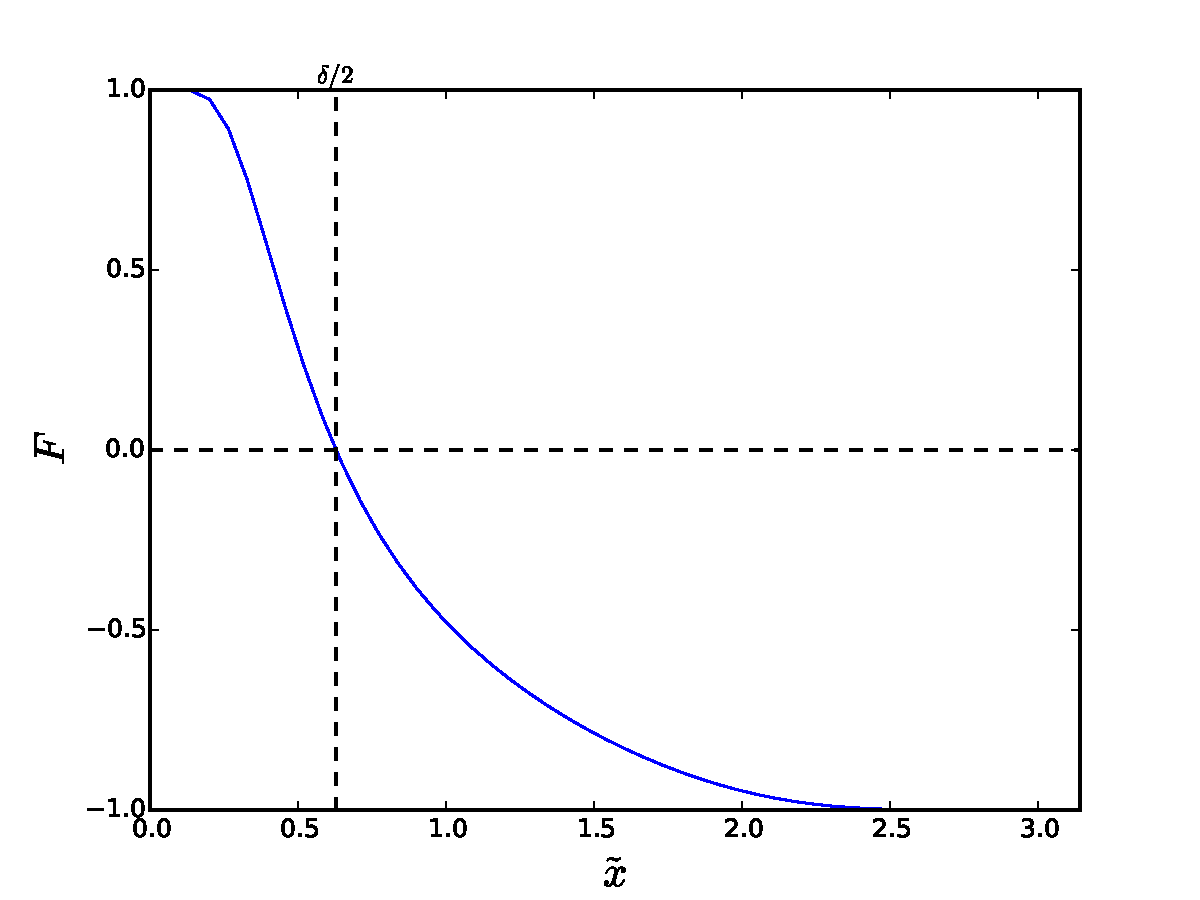
\includegraphics[width=\textwidth]{zoom_F}
  \caption[Zoom en longitude, fonction $F$]{Zoom en longitude,
    fonction $F$. Exemple pour $\delta = 2 \pi / 5$, $\tau = 3$.}
  \label{fig:zoom_F}
\end{figure}

Notons :
\begin{equation*}
  I := \int_0 ^\pi F
\end{equation*}
$I$ n'est pas calculable analytiquement. D'après l'encadrement de $F$
:
\begin{equation*}
  - \pi < I < \pi
\end{equation*}
Si $\delta = \pi$ alors :
\begin{equation*}
  F(\pi - \tilde x) = - F(\tilde x)
\end{equation*}
C'est-à-dire que $F$ est symétrique par rapport au point $(\pi / 2,
0)$. D'où :
\begin{equation*}
  \int_0 ^{\pi / 2} F = - \int_{\pi / 2} ^\pi F
\end{equation*}
et :
\begin{equation*}
  I = 0
\end{equation*}
Considérant $F$ comme une fonction de $(\tilde x, \delta, \tau)$ :
\begin{equation*}
  \forall \tilde x \in ]0, \pi[, \forall \delta \in ]0, 2 \pi[,
  \forall \tau > 0,
  \partial_\delta F(\tilde x, \delta, \tau) > 0
\end{equation*}
D'où :
\begin{equation*}
  \frac{\partial I}{\partial \delta}
  = \int_0 ^\pi \partial_\delta F\ \ud \tilde x > 0
\end{equation*}
On en déduit :
\begin{align*}
  & \delta < \pi \Rightarrow I < 0 \\
  & \delta > \pi \Rightarrow I > 0
\end{align*}
La variation de $I$ avec $\tau$ n'est pas évidente.

Posons :
\begin{equation*}
  \beta := \frac{\pi - \gamma I}{\pi - I}
\end{equation*}
On a :
\begin{equation*}
  \gamma - \beta = \frac{(\gamma - 1) \pi}{\pi - I}
\end{equation*}
donc $\beta \le \gamma$.

Posons :
\begin{equation*}
  g := \beta + (\gamma - \beta) F
\end{equation*}
On a :
\begin{equation*}
  \int_0 ^\pi g = \pi
\end{equation*}
$g$ est décroissante de $\gamma$ à $2 \beta - \gamma$. On a :
\begin{equation*}
  2 \beta - \gamma > 0
  \Leftrightarrow I < \left(\frac{2}{\gamma} - 1 \right) \pi
\end{equation*}
Puisque $I$ ne dépend pas de $\gamma$, et $I$ peut être strictement
positif et $\gamma$ peut être arbitrairement grand, cette inégalité
n'est pas forcément satisfaite. Si elle n'est pas satisfaite, il faut
diminuer $I$ ou diminuer $\gamma$. Pour diminuer $I$, on peut diminuer
$\delta$. Nous faisons dans la suite l'hypothèse supplémentaire :
\begin{equation*}
  \gamma < 2 \beta
\end{equation*}
Donc $\beta > 0$ et $g > 0$. Si $\gamma = 1$ alors :
\begin{align*}
  & \beta = 1 \\
  & g \equiv 1
\end{align*}
Si $\gamma > 1$ alors $\beta < \gamma$ et $g$ est strictement
décroissante.

On définit la fonction $x_f$ sur $\mathbb{R}$ :
\begin{equation*}
  \begin{array}{|l}
    \forall \tilde x \in [0, \pi], x_f(\tilde x) = \int_0 ^{\tilde x} g \\
    \forall \tilde x \in [- \pi, 0[, x_f(\tilde x) = - x_f(- \tilde x) \\
    \forall \tilde x \in \mathbb{R},
    x_f(\tilde x + 2 \pi) = x_f(\tilde x) + 2 \pi
  \end{array}
\end{equation*}
$x_f$ est strictement croissante sur $\mathbb{R}$.
\begin{align*}
  & x_f(- \pi) = - \pi \\
  & x_f(\pi) = \pi
\end{align*}
Cf. figure (\ref{fig:zoom_xf}).
\begin{figure}
  \centering
  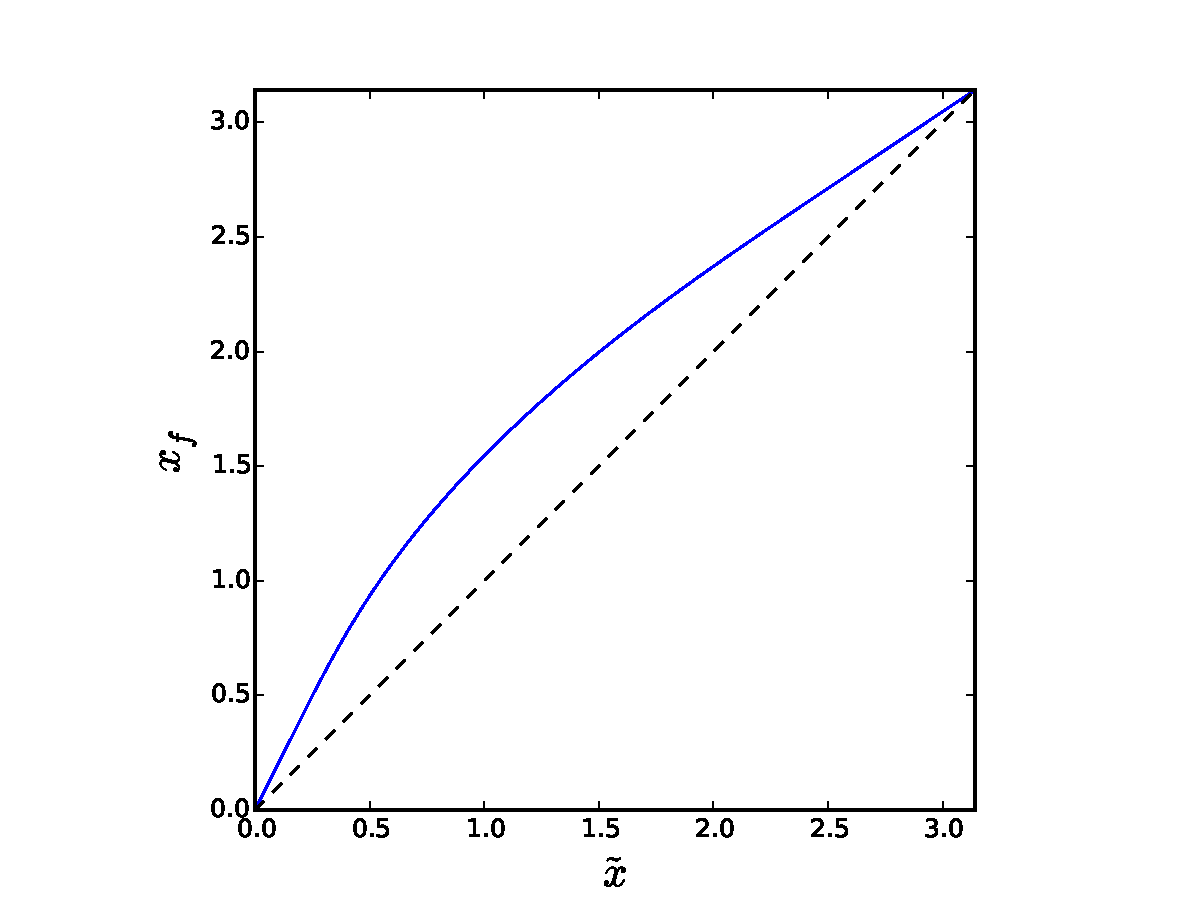
\includegraphics[width=\textwidth]{zoom_xf}
  \caption[Zoom en longitude, fonction $x_f$]{Zoom en
    longitude. Exemple pour $\delta = 2 \pi / 5$, $\tau = 3$,
    $\gamma = 2$. Le maillage zoomé est sur l'axe des abscisses. Le
    maillage uniforme est sur l'axe des ordonnées.}
  \label{fig:zoom_xf}
\end{figure}
La pente de $x_f$ en 0 est $\gamma$. Sur $\mathbb{R}$ :
\begin{equation*}
  0 < 2 \beta - \gamma \le x_f' \le \gamma
\end{equation*}
$x_f^{-1}$ est la fonction de zoom : celle qui permet de passer d'un
maillage uniforme à un maillage non uniforme. Sur $\mathbb{R}$ :
\begin{equation*}
  1 / \gamma \le (x_f^{-1})' \le \frac{1}{2 \beta - \gamma}
\end{equation*}

Si $\gamma = 1$ alors la fonction de zoom est l'identité :
\begin{align*}
  & \forall \tilde x \in \mathbb{R}, x_f(\tilde x) = \tilde x \\
  & x_f^{-1} = x_f \\
  & (x_f^{-1})' = 1
\end{align*}

\subsubsection{Discrétisation}

$N = \np{30000}$. Notons, pour $i \in \{0, \dots, N\}$ :
\begin{equation*}
  \tilde x_i = i \pi / N
\end{equation*}
et, pour $i \in \{1, \dots, N\}$ :
\begin{equation*}
  \tilde x_{i - \frac{1}{2}} = \frac{\tilde x_{i - 1} + \tilde x_i}{2}
\end{equation*}

On note :
\begin{equation*}
  h = 2 \pi / \mathtt{iim}
\end{equation*}
Soit $x_\mathrm{uv} \in [- 1 / 4, 1 / 2]$. On considère le maillage
régulier de pas $h$ :
\begin{equation*}
  y_i = - \pi + \left(i + x_\mathrm{uv} - \frac{3}{4} \right) h, i \in \mathbb{Z}
\end{equation*}
Pour $x_\mathrm{uv}$ fixé, la suite $(y_i)$ est strictement
croissante. On a :
\begin{align*}
  y_1
  & =
  - \pi + \left(x_\mathrm{uv} + \frac{1}{4} \right) \frac{2 \pi}{\mathtt{iim}} \\
  & \ge - \pi
\end{align*}
et :
\begin{align*}
  y_\mathtt{iim}
  & =
  \pi + \left(x_\mathrm{uv} - \frac{3}{4} \right) \frac{2 \pi}{\mathtt{iim}} \\
  & < \pi
\end{align*}
Donc :
\begin{align*}
  \forall i \in \{1, \dots, \mathtt{iim}\}, - \pi \le y_i < \pi
\end{align*}
Pour $i \in \{1, \dots, \mathtt{iim}\}$, on pose :
\begin{equation*}
  x_{vi} = x_f^{-1}(y_i)
\end{equation*}
Pour calculer $x_{vi}$, au lieu de résoudre directement l'équation :
\begin{equation*}
  x_f(x_{vi}) - y_i = 0
\end{equation*}
avec la fonction $x_f$, qui est lourde à calculer, on remplace $x_f$
localement par un polynôme de degré 3 interpolé, avec les bonnes
dérivées.  On a aussi besoin de :
\begin{align*}
  h (x_f^{-1})'(y_i)  & = \frac{h}{x_f'(x_{vi})} \\
  & > 0
\end{align*}

Remarquons que, puisque $x_f$ est impaire, $x_f^{-1}$ est impaire
aussi, $x_f'$ et $(x_f^{-1})'$ sont paires, donc on peut se contenter
de résoudre :
\begin{equation*}
  x_{vi} = x_f^{-1}(|y_i|)
\end{equation*}

Quand iim est grand, $h$ est petit et, pour $i \in {1, \dots,
  \mathtt{iim} - 1}$ :
\begin{equation*}
  x_{v, i + 1} - x_{vi} \approx  h (x_f^{-1})'(y_i)
\end{equation*}

Si $\gamma = 1$ alors :
\begin{equation*}
  x_{vi} = y_i
\end{equation*}

On a les correspondances données par le tableau (\ref{tab:zoom_x}).
\begin{table}
  \centering
  \begin{tabular}{l|l}
    & variable Fortran \\
    \hline
    $\gamma$ & grossismx \\
    $N$ & nmax \\
    $\tilde x_i$ & xtild(i) \\
    $\tilde x_{i - \frac{1}{2}}$ & xmoy(i) \\
    $F(\tilde x_i)$ & fhyp(i) \\
    $F(\tilde x_{i - \frac{1}{2}})$ & fxm(i) \\
    $\int_0 ^{\tilde x_i} F \ud \tilde x$ & ffdx(i) \\
    $g(\tilde x_i)$ & g(i) \\
    $x_f(\tilde x_i)$ & xf(i) \\
    $y_i$ & y \\
    $x_{vi}$ & xvrai(i) \\
    $x_f'(x_{vi}) = g(|x_{vi}|)$ & gvrai(i) \\
    $h \times (x_f^{-1})'(y_i)$ & xprim(i)
  \end{tabular}
  \caption{Zoom en longitude. Correspondances entre objets
    mathématiques et variables Fortran dans les procédures fxhyp et
    invert\_zoom\_x.}
  \label{tab:zoom_x}
\end{table}

\section{Filtre}

Principe du filtrage : décomposition d'un champ en harmoniques
sphériques et conservation d'une partie seulement du
spectre. Références : Umscheid (1971 k0904), Gates (1971 k0905), Sadourny
(1975 k0914), Kasahara (1977 k0907, § V.E), Sharma (1986 k0918).

Arbres des appels partiels :
\begin{verbatim}
 inifilr
 . inifgn
 . inifilr_hemisph
\end{verbatim}
\begin{verbatim}
 filtreg_scal
 . filtreg_hemisph
\end{verbatim}
\begin{verbatim}
filtreg_v
 . filtreg_hemisph
\end{verbatim}

\subsection{Procédure inifgn}

Cette procédure calcule les valeurs propres et les vecteurs propres de
l'analogue discret de $\frac{\partial^2}{\partial \lambda^2}$.

Remarque. Dans l'espace des fonctions $\mathscr{C}^\infty$ sur
$\mathbb{R}$, dont $2 \pi$ est une période, les valeurs propres de la
dérivée seconde sont :
\begin{equation*}
  - k^2, k \in \mathbb{N}
\end{equation*}
Vecteur propre associé à 0 : fonction constante. Vecteur propre
associé à $- k^2$ pour $k \ge 1$ :
\begin{equation*}
  f(\lambda) = a \cos k \lambda + b \sin k \lambda
\end{equation*}

L'analogue discret de $\frac{\partial^2}{\partial
  \lambda^2}$ est une matrice de différentiation $\Delta$.  On peut
choisir $\Delta$ pour un maillage uniforme puis appliquer une
transformation pour passer à un maillage non uniforme. Cf. Kitson
(2003 k0911, § 4).

Notons $n = \mathtt{iim}$,
\begin{equation*}
  h = 2 \pi / n
\end{equation*}
et :
\begin{equation*}
  A = \frac{1}{h}
  \begin{bmatrix}
    -1 & 1 \\
    & -1 & \ddots \\
    & & \ddots & 1 \\
    1 & & & -1
  \end{bmatrix}  
\end{equation*}
(les valeurs non marquées et en dehors des points de suspension sont
nulles), matrice de taille $n$.

\subsubsection{Maillage uniforme}

Pour des dérivées centrées sur un maillage uniforme, la matrice
donnant la dérivée aux longitudes des points u est :
\begin{equation*}
  D_u = A
\end{equation*}
On peut appliquer $D_u$ à un champ défini aux longitudes des
scalaires. La matrice donnant la dérivée aux longitudes des points v
est :
\begin{equation*}
  D_v = - \ltrans{A} = \frac{1}{h}
  \begin{bmatrix}
    1 & & & - 1 \\
    - 1 & \ddots \\
    & \ddots & \ddots \\
    & & - 1 & 1
  \end{bmatrix}
\end{equation*}
On peut appliquer $D_v$ à un champ défini aux longitudes des points
u. La matrice donnant la dérivée seconde aux longitudes des points v
est alors :
\begin{equation*}
  \Delta_v = D_v D_u = \frac{1}{h^2}
  \begin{bmatrix}
    - 2 & 1 & & 1 \\
    1 & \ddots & \ddots \\
    & \ddots & \ddots & 1 \\
    1 & & 1 & - 2
  \end{bmatrix}
\end{equation*}
Cf. par exemple Sfakianakis (2009 k0912, § 1.3.2). On peut appliquer
$\Delta_v$ à un champ défini aux longitudes des scalaires. De même :
\begin{equation*}
  \Delta_u = D_u D_v
\end{equation*}
$A$ et $\ltrans{A}$ sont circulantes donc elles commutent. D'où :
\begin{equation*}
  \Delta_u = \Delta_v =: \Delta
\end{equation*}
$\Delta$ est symétrique réelle donc diagonalisable avec des valeurs
propres réelles (théorème spectral). 0 est une valeur proopre de
$\Delta$ (vecteur propre : matrice colonne ne contenant que des
1). Les valeurs propres de $\Delta$ sont négatives ($- \Delta$ est
positive, étant le produit d'une matrice et de sa transposée, cf. par
exemple Horn (2012 k0915, théorème 7.2.7) ou Voedts (2002 k0916, exercice
13-3.18)). Et même : les valeurs propres sont comprises entre $- 4 /
h^2$ et 0 (théorème de Gerschgorin). On peut même trouver l'expression
analytique des valeurs propres en utilisant les propriétés des
matrices circulantes :
\begin{equation*}
  - h^2 \Delta = C(2, -1, 0, \dots, 0, - 1)
\end{equation*}
Notons $P$ le polynôme :
\begin{equation*}
  P(X) = 2 - X - X^{n - 1}
\end{equation*}
et $\omega$ la racine n-ième de l'unité :
\begin{equation*}
  \omega = \exp(2 i \pi / n)
\end{equation*}
Les valeurs propres de $C(2, -1, 0, \dots, 0, - 1)$ sont :
\begin{equation*}
  \lambda_k = P(\omega^k), \qquad k = 0, \dots, n - 1
\end{equation*}
Explicitons :
\begin{align*}
  \lambda_k & = 2 - \omega^k - \omega^{k n - k} \\
  & = 2 - \omega^k - \omega^{- k} \\
  & = 2 - \exp(2 i \pi k / n) - \exp(- 2 i \pi k / n) \\
  & = 2 \left(1 - \cos \frac{2 \pi k}{n} \right) \\
  & = 4 \sin^2 \frac{\pi k}{n}
\end{align*}
Si $n$ est pair alors les valeurs propres pour $k = 0, \dots, n / 2$
sont distinctes, et les valeurs propres suivantes les répètent :
\begin{equation*}
  \forall k \in \left\{\frac{n}{2} + 1, \dots, n - 1 \right\},
  \lambda_k = \lambda_{n - k}
\end{equation*}
La plus grande valeur propre est :
\begin{equation*}
  \lambda_{n / 2} = 4
\end{equation*}
Les valeurs propres de $\Delta$ sont $- \lambda_k / h^2$. Remarquons
la relation avec les valeurs propres de la dérivée seconde continue :
\begin{equation*}
  - \lambda_k / h^2 = - \left(\sinc \frac{\pi k}{n} \right)^2 k^2
\end{equation*}

\subsubsection{Maillage non uniforme}
\label{sec:non_uniform}

Notons $y_{i + \frac{1}{2}}$ les points de la grille uniforme
correspondant aux longitudes u. Posons :
\begin{equation*}
  s_{ui} := (x_f^{-1})'(y_{i + \frac{1}{2}})
\end{equation*}
($s_{ui} \ge 1 / \gamma$, $h s_{ui}$ est donnée par la variable Fortran
xprimu). Notons $S_u$ la matrice diagonale dont les éléments diagonaux sont
les $s_{ui}$ :
\begin{equation}
  \label{eq:S_u}
  S_u = \mathrm{diag}(s_u)
\end{equation}

De même, notons $y_i$ les points de la grille uniforme correspondant
aux longitudes v. Posons :
\begin{align}
  \notag
  & s_{vi} := (x_f^{-1})'(y_i) \\
  \label{eq:S_v}
  & S_v = \mathrm{diag}(s_v)
\end{align}
($s_{vi} \ge 1 / \gamma$, $h s_{vi}$ est donnée par la variable Fortran
xprimv).

\paragraph{Transformation simple.}

Pour passer à un maillage non uniforme, en appliquant simplement la
transformation de maillage, on remplacerait simplement $h$ dans $D_u$
par $h (x_f^{-1})'$ aux points u. On obtiendrait :
\begin{equation*}
  D_u = S_u^{-1} A
\end{equation*}
C'est-à-dire, en dehors des bords, en appliquant la dérivée à la
température par exemple :
\begin{equation*}
  (D_u T)_i = \frac{T_{i + 1} - T_i}{h s_{ui}}
\end{equation*}
Et :
\begin{equation*}
  D_v = - S_v^{-1}\ \ltrans{A}
\end{equation*}
C'est-à-dire, en dehors des bords, en appliquant la dérivée au vent
zonal par exemple :
\begin{equation*}
  (D_v u)_i = \frac{u_i - u_{i - 1}}{h s_{vi}}
\end{equation*}
D'où :
\begin{align}
  \label{eq:delta_v_simple}
  & \Delta_v = D_v D_u = - S_v^{-1}\ \ltrans{A} S_u^{-1} A \\
  \notag
  & \Delta_u = D_u D_v = - S_u^{-1} A S_v^{-1}\ \ltrans{A}
\end{align}
Cf. Kitson (2003 k0911, § 4). Ce qui donnerait, par exemple sur $T$ :
\begin{equation*}
  (\Delta_v T)_i
  =
  \frac{1}{h^2 s_{vi}}
  \left[
    \frac{T_{i - 1}}{\sqrt{r_{i - 1}}}
    - \left(\frac{1}{r_{i - 1}} + \frac{1}{s_{ui}} \right) T_i
    + \frac{T_{i + 1}}{\sqrt{r_{i + 1}}}
  \right]
\end{equation*}

\paragraph{Transformation sophistiquée.}

Mais ce qui est fait dans inifgn est plus sophistiqué :
\begin{equation*}
  D_u = S_u^{- 1 / 2} A S_v^{- 1 / 2}
\end{equation*}
C'est-à-dire, en dehors des bords, en appliquant la dérivée à la
température par exemple :
\begin{equation*}
  (D_u T)_i
  = \frac{1}{h \sqrt{s_{ui}}}
  \left(\frac{T_{i + 1}}{\sqrt{s_{i + 1}}} - \frac{T_i}{\sqrt{s_{vi}}} \right)
\end{equation*}
Et :
\begin{equation*}
  D_v = - \ltrans{D_u} = - S_v^{- 1 / 2}\ \ltrans{A} S_u^{- 1 / 2}
\end{equation*}
C'est-à-dire, en dehors des bords, en appliquant la dérivée au vent
zonal par exemple :
\begin{equation*}
  (D_v u)_i
  = \frac{1}{h \sqrt{s_{vi}}}
  \left(\frac{u_i}{\sqrt{s_{ui}}} - \frac{u_{i - 1}}{\sqrt{r_{i - 1}}} \right)
\end{equation*}
Et toujours :
\begin{align*}
  & \Delta_v = D_v D_u \\
  & \Delta_u = D_u D_v
\end{align*}
$\Delta_v$ et $\Delta_u$ sont chacune symétriques. Explicitons, par
exemple sur $T$ et $u$. Pour cela, nous pouvons remarquer :
\begin{align*}
  & \Delta_v = - S_v^{- 1 / 2} (\ltrans{A} S_u^{- 1} A)  S_v^{- 1 / 2} \\
  & \Delta_u = - S_u^{- 1 / 2} (A S_v^{- 1}\ \ltrans{A}) S_u^{- 1 / 2}
\end{align*}
D'où :
\begin{equation*}
  (\Delta_v T)_i
  =
  \frac{1}{h^2}
  \left[
    \frac{T_{i - 1}}{r_{i - 1} \sqrt{s_{i - 1} s_{vi}}}
    - \frac{T_i}{s_{vi}} \left(\frac{1}{r_{i - 1}} + \frac{1}{s_{ui}} \right)
    + \frac{T_{i + 1}}{s_{ui} \sqrt{s_{vi} s_{i + 1}}}
  \right]
\end{equation*}
\begin{equation*}
  (\Delta_u u)_i
  =
  \frac{1}{h^2}
  \left[
    \frac{u_{i - 1}}{s_{vi} \sqrt{r_{i - 1} s_{ui}}}
    - \frac{u_i}{s_{ui}} \left(\frac{1}{s_{vi}} + \frac{1}{s_{i + 1}} \right)
    + \frac{u_{i + 1}}{s_{i + 1} \sqrt{s_{ui} r_{i + 1}}}
  \right]
\end{equation*}

Les valeurs propres de $\Delta_v$ et $\Delta_u$ sont négatives ($-
\Delta_v$ et $- \Delta_u$ sont positives, chacune étant le produit
d'une matrice et de sa transposée). 0 est une valeur propre de
$\Delta_v$ et $\Delta_u$ (le déterminant de $A$ est nul donc aussi
celui de $\Delta_v$ et $\Delta_u$).

Remarque. On peut regarder les bornes données par le théorème de
Gershgorin. Pour $- h^2 \Delta_u$ par exemple, l'intervalle de
Gershgorin à la ligne $i$ est :
\begin{equation*}
  \frac{1}{s_{ui}} \left(\frac{1}{s_{vi}} + \frac{1}{s_{i + 1}} \right)
  \pm
  \left(
    \frac{1}{s_{vi} \sqrt{r_{i - 1} s_{ui}}}
    + \frac{1}{s_{i + 1} \sqrt{s_{ui} r_{i + 1}}}
  \right)
\end{equation*}
Si $\gamma > 1$, $(x_f^{-1})'$ est strictement décroissant sur $[-
\pi, 0]$ et strictement décroissant sur $[0, \pi]$. Donc l'ordre des
$s_{vi}$ et des $s_{ui}$ peut être quelconque. L'intervalle passe en dessous
de 0 si :
\begin{equation*}
  \frac{1}{\sqrt{s_{ui}}} \left(\frac{1}{s_{vi}} + \frac{1}{s_{i + 1}} \right)
  < \frac{1}{s_{vi} \sqrt{r_{i - 1}}} + \frac{1}{s_{i + 1} \sqrt{r_{i + 1}}} 
\end{equation*}
Je vérifie sur un maillage particulier qu'au moins un des intervalles
passe en dessous de 0 (cf. script \verb+inifgn.py+). Par ailleurs,
puisque les $s_{ui}$ et les $s_{vi}$ sont supérieurs à $1 / \gamma$, les
valeurs propres de $- h^2 \Delta_u$ sont inférieures à $4
\gamma^2$. Les valeurs propres de $\Delta_v$ et $\Delta_u$ sont
comprises entre $- 4 \gamma^2 / h^2$ et 0.

inifgn calcule les valeurs propres $e$ de $\Delta_v$ et les vecteurs
propres $\Lambda_u$ et $\Lambda_v$ de $\Delta_u$ et
$\Delta_v$. $\Lambda_u$ et $\Lambda_v$ sont orthogonales. On a
donc :
\begin{equation*}
  \ltrans{\Lambda_v} \Delta_v \Lambda_v = \mathrm{diag}(e)
\end{equation*}
Pour une grille régulière en longitude : $\Lambda_v = \Lambda_u$.

Remarque :
\begin{equation*}
  S_v^{- 1 / 2} \Delta_v S_v^{1 / 2} = - S_v^{-1}\ \ltrans{A} S_u^{-1} A
\end{equation*}
Cf. équation (\ref{eq:delta_v_simple}). Et on a une équation analogue
pour $\Delta_u$.

\subsection{Procédure inifilr}

Rappel de notation : $n$ := iim.

Détermination de jfilt[ns][uv]. Pour une grille régulière en latitude,
nous pourrions chercher jfilt[ns][uv] à partir de jjm / 2
environ. Cf. figure (\ref{fig:jfilt}). Mais pour tenir compte d'une
grille irrégulière en latitude, mieux vaut chercher l'indice
correspondant à l'équateur (variable j1). j1 pour rlatu est toujours
inférieur à jjm + 1 puisque rlatu(jjm + 1) == $- \pi / 2$. Si j1 pour
rlatv vaut jjm + 1 alors matricevs est vide et jfiltsv = jjm + 1.

\begin{equation*}
  \mathtt{colat0}
  = \min\left[1/2, \frac{\min \delta \phi_u}{\min (h s_u)} \right]
\end{equation*}
\begin{equation*}
  \mathtt{rlamda} = \frac{2 \gamma}{h \sqrt{-e} \times \mathtt{colat0}}
\end{equation*}
D'après le § \ref{sec:non_uniform} :
\begin{equation*}
  e_n \ge - 4 \gamma^2 / h^2
\end{equation*}
donc :
\begin{equation}
  \label{eq:rlamda}
  \mathtt{rlamda}_n \ge 1 / \mathtt{colat0}
\end{equation}

La procédure calcule :
\begin{align*}
  & M_u = \Lambda_v (\mathrm{diag}(\alpha_u) - I)\ \ltrans{\Lambda_v} \\
  & M_v = \Lambda_u (\mathrm{diag}(\alpha_v) - I)\ \ltrans{\Lambda_u}
\end{align*}
où $\alpha_u$ et $\alpha_v$ sont donnés par l'équation
(\ref{eq:alpha}) aux latitudes rlatu et rlatv.

Pour une grille régulière en longitude :
\begin{equation*}
  e_n = - 4 / h^2
\end{equation*}
donc :
\begin{equation*}
  1 / \mathtt{rlamda}(n) = \mathtt{colat0}
\end{equation*}
Pour une grille régulière en longitude et latitude :
\begin{equation*}
  \mathtt{colat0}
  = \min\left(1/2, \frac{n}{2 \times \mathtt{jjm}} \right)
\end{equation*}

\subsection{Procédure inifilr\_hemisph}

Pour chaque latitude $\phi$ reçue, on pose :
\begin{align}
  \notag
  & \alpha_1 := 1 \\
  \label{eq:alpha}
  & \mathrm{pour}\ i \in \{2, \dots, n\}, \alpha_i
  := \min
  \left(1, \frac{2 \gamma \cos \phi}{\sqrt{- e_i} h\ \mathtt{colat0}} \right)
\end{align}
On a :
\begin{equation*}
  \forall i, \alpha_i \in ]0, 1]
\end{equation*}
et les $\alpha_i$ sont décroissants. $\alpha_i$ pour $i \ge 2$ est
donné en Fortran par :
\begin{verbatim}
min(1., rlamda(i) * cos(rlat))
\end{verbatim}
Les latitudes reçues sont dans l'ordre croissant. La procédure peut
donc chercher l'indice jfilt de la première latitude, si elle existe,
pour laquelle $\alpha_n < 1$. Si une telle latitude est trouvée, alors
jfilt est inférieur à \verb+n_lat+ et, pour chaque latitude d'indice
supérieur à jfilt, il existe un premier indice modfrst $\in \{2,
\dots, n\}$ tel que $\alpha_\mathrm{modfrst} < 1$.

Remarque. Si jfilt existe alors :
\begin{equation*}
  \cos \phi_\mathtt{jfilt} < 1 / \mathtt{rlamda}(n)
\end{equation*}
D'où, avec l'inégalité (\ref{eq:rlamda}) :
\begin{equation*}
  \cos \phi_\mathtt{jfilt} < \mathtt{colat0}
\end{equation*}
Donc pour les latitudes d'indice supérieur à jfilt :
\begin{equation*}
  \cos \phi < \mathtt{colat0}
\end{equation*}

Pour une grille régulière en latitude et longitude, avec iim $\ge$
jjm, on a les simplifications suivantes. Pour $i \in \{2, \dots, n\}$
:
\begin{equation*}
  \alpha_i
  = \min \left(1, \frac{4 \cos \phi}{\sqrt{- e_i} h} \right)
\end{equation*}
De plus :
\begin{equation*}
  e_n = - 4 / h^2
\end{equation*}
donc :
\begin{equation*}
  \alpha_n = \min(1, 2 \cos \phi)
\end{equation*}
jfilt est l'indice de la première latitude, si elle existe, pour
laquelle $\cos \phi < 1 / 2$.

Notons $\Lambda$ la matrice de vecteurs propres reçue. Pour chaque
latitude d'indice supérieur à jfilt, la procédure calcule :
\begin{equation*}
  M = \Lambda (\mathrm{diag}(\alpha) - I)\ \ltrans{\Lambda}
\end{equation*}
(variable Fortran matrice). Les éléments de $\mathrm{diag}(\alpha) -
I$ valent 0 jusqu'à l'indice modfrst - 1, et ils sont dans $]-1, 0[$
ensuite.

Remarque. Si jfilt vaut \verb+n_lat+ + 1 alors matrice et matrinv sont
vides.

Remarque. Ne pas sélectionner les latitudes à filtrer ne changerait
rien aux résultats. Pour les latitudes d'indice strictement inférieur
à jfilt, $\alpha \equiv 1$ et $M = 0$. Mais ce serait une perte de
temps de calcul puisque les procédures \verb+filtreg_scal+ et
\verb+filtreg_v+ s'appliqueraient à ces latitudes avec des matrices de
filtrage nulles. En d'autres termes, la sélection du filtrage est
entièrement dans l'équation (\ref{eq:alpha}). Les latitudes d'indice
supérieur à jfilt sont simplement celles pour lesquelles il existe
au moins un mode à filtrer.

\subsection{Procédures filtreg\_scal et filtreg\_v}

\`A une latitude donnée, notons $M_u$ et $M_v$ les matrices de
filtrage (matriceu[ns] et matricev[ns]à la latitude
considérée). Reprenons aussi les notations (\ref{eq:S_u}) et
(\ref{eq:S_v}) pour $S_u$ et $S_v$. Notons $I$ la matrice identité de
taille $n$. Pour les latitudes à filtrer seulement, on définit quatre
filtres :
\begin{itemize}
\item grille des scalaires, champ intensif :
  \begin{equation}
    \label{eq:filter_scal_intensive}
    \mathscr{F}_\mathrm{scal} = I + S_v^{-1/2} M_u S_v^{1/2}
  \end{equation}
\item grille des scalaires, champ extensif :
  \begin{equation}
    \label{eq:filter_scal_extensive}
    \mathscr{F}^*_\mathrm{scal} = I + S_v^{1/2} M_u S_v^{- 1/2}
  \end{equation}
\item grille de la vorticité, champ intensif :
  \begin{equation}
    \label{eq:filter_vort_intensive}
    \mathscr{F}_\mathrm{vort} = I + S_u^{-1/2} M_v S_u^{1/2}
  \end{equation}
\item grille de la vorticité, champ extensif :
  \begin{equation}
    \label{eq:filter_vort_extensive}
    \mathscr{F}^*_\mathrm{vort} = I + S_u^{1/2} M_v S_u^{- 1/2}
  \end{equation}
\end{itemize}
(Rappel : pour $n$ grand, $h s_{vi} \approx (\delta \lambda)_i$.)

Notons $\psi_i$ le champ à filtrer, à une latitude et un niveau
vertical donnés, où $i$ est l'indice de longitude. Notons $\psi$ la
matrice colonne des $\psi_i$. Pour les latitudes à filtrer seulement
et pour tous les niveaux verticaux du champ reçu, les procédures
calculent $\mathscr{F}_\mathrm{scal} \psi$,
$\mathscr{F}_\mathrm{scal}^* \psi$, $\mathscr{F}_\mathrm{vort} \psi$
ou $\mathscr{F}_\mathrm{vort}^* \psi$.

Les matrices $M_u$ et $M_v$ sont symétriques donc :
\begin{align*}
  & \mathscr{F}^*_\mathrm{scal} = \ltrans{\mathscr{F}_\mathrm{scal}} \\
  & \mathscr{F}^*_\mathrm{vort} = \ltrans{\mathscr{F}_\mathrm{vort}}
\end{align*}

En principe, le lissage doit s'opérer sur un champ intensif. \`A
partir d'un champ extensif, on doit calculer le champ intensif
correspondant. Pour illustrer, on peut considérer un filtrage extrême
qui remplacerait un champ intensif par sa moyenne :
\begin{align*}
  \bar \psi & = \frac{1}{2 \pi} \sum_i (\delta \lambda)_i \psi_i \\
  & = \psi_i + \frac{1}{2 \pi} \sum_{j \ne i} (\delta \lambda)_j \psi_j
  + \left[\frac{ (\delta \lambda)_i}{2 \pi} - 1\right] \psi_i
\end{align*}
Pour un champ extensif, on écrirait :
\begin{equation*}
  \frac{\bar \psi_i}{(\delta \lambda)_i} = \frac{1}{2 \pi}\sum_j \psi_j
\end{equation*}
De manière générale, si on sait comment filtrer un champ intensif, on
sait comment filtrer un champ extensif $\psi$ : on filtre $S^{-1}
\psi$ puis on revient au champ extensif en multipliant par $S$. Il
faut donc que :
\begin{align*}
  & \mathscr{F}^*_\mathrm{scal} = S_v \mathscr{F}_\mathrm{scal} S_v^{-1} \\
  & \mathscr{F}^*_\mathrm{vort} = S_u \mathscr{F}_\mathrm{vort} S_u^{-1}
\end{align*}
ce qui est bien vérifié par les définitions
(\ref{eq:filter_scal_intensive}) à (\ref{eq:filter_vort_extensive}).

On voit que, par exemple :
\begin{equation*}
  \mathscr{F}_\mathrm{scal} T
  =
  S_v^{-1/2} \Lambda_v \mathrm{diag}(\alpha_u)\ \ltrans{\Lambda_v} S_v^{1/2} T
\end{equation*}
Ainsi, le filtre lisse $S_v^{1/2} T$. En effet, $\ltrans{\Lambda_v}$
est la matrice de passage de la base canonique à la base des vecteurs
propres. La multiplication par $\mathrm{diag}(\alpha_u)$ réduit les
modes propres correspondant aux plus grandes valeurs propres. La
multiplication par $\Lambda_v$ ramène dans la base canonique.

Reste à comprendre l'équation (\ref{eq:alpha}) et pourquoi on ne lisse
pas simplement $T$.

Pour une grille régulière en longitude :
\begin{align*}
  & \mathscr{F}^*_\mathrm{scal} = \mathscr{F}_\mathrm{scal}
  = \Lambda \mathrm{diag}(\alpha_u)\ \ltrans{\Lambda} \\
  & \mathscr{F}^*_\mathrm{vort} = \mathscr{F}_\mathrm{vort}
  = \Lambda \mathrm{diag}(\alpha_v)\ \ltrans{\Lambda}
\end{align*}
D'où :
\begin{equation*}
  \Delta \mathscr{F}_\mathrm{scal}
  = \Lambda \mathrm{diag}(e) \mathrm{diag}(\alpha_u)\ \ltrans{\Lambda}
\end{equation*}

\subsection{Procédure filtreg\_hemisph}

Notons $\psi_i$ le champ à filtrer, à une latitude et un niveau
vertical donnés, où $i$ est l'indice de longitude. Notons $\psi$ la
matrice colonne des $\psi_i$. Notons la $D$ la matrice diagonale de
diagonale sdd. Pour toutes les latitudes et tous les niveaux verticaux
du champ reçu, la procédure calcule :
\begin{equation*}
  \psi = \psi + D^{-1} M D  \psi
\end{equation*}
où $M$ est la matrice de filtrage reçue, à la latitude et au niveau
vertical considérés.

\section{Les traceurs en général}

Procédures qui concernent les traceurs dans le programme
\verb+ce0l+ : \verb+infotrac_init+, \verb+etat0dyn+. Procédures qui
concernent les traceurs dans le programme \verb+gcm+ :
\verb+infotrac_init+, \verb+dynetat0+, \verb+caladvtrac+, \verb+advtrac+,
\verb+physiq+, \verb+phytrac+. Laurent L. connaît peut-être bien le
traitement des traceurs. Il a écrit une grande partie de la
``physique'' du modèle.

Dans le fichier \verb+traceur.def+, le premier nombre est le nombre de
traceurs. Chaque ligne suivante correspond à un traceur. Pour chaque
traceur, on indique le numéro du schéma
d'advection à utiliser. Les numéros sont définis dans
\verb+infotrac_init+.

\verb+traceur.def+ est lu uniquement dans le sous-programme
\verb+infotrac_init+. \verb+infotrac_init+ impose que \verb+nqmx+ soit égal
au nombre de traceurs indiqué dans \verb+traceur.def+. \verb+physiq+
impose \verb+nqmx+ $\ge 2$. \verb+nbtr+ (variable de \verb+dimphy+)
vaut 1 pour \verb+nqmx+ \verb+=+ \verb+2+ et \verb+nqmx+ -- \verb+2+
pour \verb+nqmx+ $\ge 3$.  \verb+nqmx-2+ est passé à \verb+phytrac+ et
devient \verb+nq_phys+ dans \verb+phytrac+. \verb+initrrnpb+ impose
\verb+nbtr+ $\ge 2$, mais il n'est appelé que si \verb+rnpb+ est vrai.
Cf. aussi message de Ionela M. du 29/11/6.

\verb+phytrac+ peut effectuer un traitement spécial pour les traceurs
plomb et radon (décroissance radioactive etc.).  \verb+phytrac+
suppose que ce sont les traceurs numérotés 3 et 4. Donc si on veut
laisser les traceurs plomb et radon, avec le traitement spécial qui
leur est réservé, il faut les laisser en troisième et quatrième
position dans \verb+traceur.def+ et laisser \verb+rnpb+ à
\verb+.true.+ dans \verb+physiq+. Cette variable est définie dans
\verb+physiq+ et \verb+phytrac+ uniquement. Cf. le message de Frédéric
H. du 26/1/7.

Dans le programme \verb+ce0l+, la variable qui contient la
distribution initiale des traceurs est \verb+q+. Cette variable est
définie dans \verb+etat0dyn+. Pour la vapeur d'eau (traceur numéro 1), la
distribution initiale est calculée à partir de la variable \verb+R+ du
fichier \verb+ECDYN.nc+. Cf. figure (\ref{fig:ECDYN}). La
distribution initiale des traceurs est écrite dans \verb+restart.nc+.

Dans le programme \verb+gcm+, la procédure \verb+infotrac_init+ lit les
noms des traceurs. La procédure \verb+dynetat0+ lit les distributions
initiales à partir du fichier \verb+start.nc+ vers la variable
\verb+q+. Cette variable se retrouve intacte dans \verb+leapfrog+. Par
ailleurs, la concentration de radon dans le sol est lue dans
\verb+startphy.nc+ par \verb+phytrac+. Dans \verb+phytrac+, on calcule
la fraction massique à $t + \ud t$ :
\begin{displaymath}
  q(\vec r, t + \ud t) = q(\vec r, t) + (\partial_t q)(\vec r, t)\ud t
\end{displaymath}
Cf. figure (\ref{fig:Traceurs}).
\begin{figure}
  \centering
  \includegraphics{Traceurs}
  \caption{Flot de données concernant les traceurs.}
  \label{fig:Traceurs}
\end{figure}
Les distributions de traceurs calculées sont écrites dans
\verb+dyn_hist.nc+ et \verb+histins.nc+. Les distributions finales
sont écrites dans \verb+restart.nc+ par \verb+dynredem1+. Par
ailleurs, la concentration de radon dans le sol est écrite dans
\verb+restartphy.nc+ par \verb+phytrac+.

Si on encadre les valeurs de l'abondance d'un traceur, on fausse le
bilan de masse pour ce traceur.

Cf. \href{../Ozone_texfol/ozone.pdf}{documentation sur le traitement
  de l'ozone}.

Dans la mesure où on a souhaité regrouper tous les appels physiques
pour les traceurs dans phytrac, les flux de masse et coefficients
d'échange sont calculés à des moments différents de la physique, donc
pour des champs de température différents. Donc passer t ou
\verb+t_seri+ est sans doute assez indifférent.

\section{Procédure \texttt{bilan\_dyn}}

\verb+bilan_dyn+ est toujours lancé sur un état issu d'un pas
leapfrog, juste avant un pas Matsuno. S'il y a un appel de la physique
à ce pas de temps alors \verb+bilan_dyn+ est après l'appel de la
physique. Il peut ne pas y avoir d'appel de la physique à ce pas de
temps si iphysiq est différent de iperiod. Cf. § \ref{sec:time}.

Calcul de la moyenne zonale et temporelle du transport. Les moyennes
sont à niveau hybride $s$ constant, pondérées par l'épaisseur des
couches. Cf.
\hyperref{../../../../Apprentissage/Climate/Meridional_transport_texfol/meridional_transport.pdf}{sec}{moyenne_s_constant}{Système
  climatique – Transport méridien, § Moyennes zonales à coordonnée
  verticale hybride constante}. \verb+bilan_dyn+ écrit dans
\verb+dynzon.nc+.

Notons $Y$ la coordonnée équivalente à $\phi$, qui est discrétisée
régulièrement. Cf. \href{../../../Documentation_LMDZ/Dynamics_texfol/dynamics.pdf}{Discrétisation
  des équations de la dynamique dans le modèle LMDZ}. Notons $\ud^2 S$
l'élément de surface sur un cône à une latitude donnée. La variable
Fortran pbarv est calculée par la procédure flumass :
\begin{align*}
  \mathtt{pbarv} & = \rho\ \ud^3 \tau\ v_\mathrm{contravariant} \\
  & = \rho\ \ud^3 \tau\ \frac{v}{a} \frac{\ud Y}{\ud \phi} \\
  & = \rho v (a \cos \phi\ \ud \lambda\ \ud z) \ud Y \\
  & = \rho v\ \ud^2 S\ \ud Y \\
  & = \frac{a \cos \phi}{g} v (\partial_s p)\ \ud \lambda\ \ud Y\ \ud s
\end{align*}
\`A strictement parler, pbarv ne représente donc pas le flux de masse
à travers $\ud^2 S$, qui serait $\rho v\ \ud^2 S$, mais ce flux
multiplié par $\ud Y$.

Dans \verb+dynzon.nc+, les variables NetCDF ont des
noms qui contiennent les chaînes de caractères suivantes :
\begin{description}
\item[TOT] : pour la circulation totale $[\overline{vq}]$
\item[MMC] : pour mean meridional circulation $[\bar v] [\bar q]$
\item[TRS] : pour les transitoires
  \begin{equation*}
    [\overline{v' q'}] = [\overline{v q}] - [\bar v \bar q]
  \end{equation*}
\item[STN] : pour les stationnaires
  \begin{equation*}
    [\bar v^* \bar q^*] = [\bar v \bar q] - [\bar v] [\bar q]
  \end{equation*}
\end{description}
Cf. par exemple tableau \ref{tab:variables_bilan_dyn} pour le
transport de température.
\begin{table}
  \centering
  \begin{tabular}{lll}
    Variable NetCDF & Variable Fortran & Définition \\
    \hline
                    & \verb+masse_cum+, 2
                                       & $\frac{a^2 \cos \phi}{g}
                                         \langle \partial_s p \rangle_t
                                         \ \ud \lambda\ \ud \phi\ \ud s$ \\
    & zmasse & $\ud \phi\ \ud s\ \frac{a^2 \cos \phi}{g}
    \int \langle \partial_s p \rangle_t\ \ud \lambda$ \\
                    & \verb+q_cum(:, :, :, 1)+ & $\bar T$ \\
    \verb+T+ & \verb+vq(:, :, iave, 1)+ & $[\bar T]$ \\
    \verb+TOTvT+ & \verb+vq(:, :, itot, 1)+ & $[\overline{v T}]$ \\
                    & \verb+flux_vq_cum(:, :, :, 1)+
                                       & $\frac{a \cos \phi}{g}
                                         \langle v T \partial_s p \rangle_t
                                         \ \ud \lambda\ \ud Y\ \ud s$ \\
    \verb+MMCvT+ & \verb+vq(:, :, immc, 1)+ & $[\bar v] [\bar T]$ \\
                    & \verb+flux_v_cum(:, :, :, 1)+
                                       & $\frac{a \cos \phi}{g}
                                         \langle v \partial_s p \rangle_t
                                         \ \ud \lambda\ \ud Y\ \ud s$ \\
                    & v, 1
                                       & $\ud Y\ \ud s\ \frac{a\cos \phi}{g}
    \int \langle v \partial_s p \rangle_t\ \ud \lambda$ \\
    v & v, 2 & $[\bar v]$ \\
    & qy, iq = 1 & $\langle T \partial_s p \rangle_t \frac{a^2 \cos \phi}{g}
                   \ \ud \lambda\ \ud \phi\ \ud s$ \\
    & vqtmp, iq = 1 & $[\bar v \bar T]$ \\
    \verb+TRSvT+ & \verb+vq(:, :, itrs, 1)+
    & $[\overline{v T}] - [\bar v \bar T]$ \\
    \verb+STNvT+ & \verb+vq(:, :, istn, 1)+
                                       & $[\bar v \bar T] - [\bar v] [\bar T]$
  \end{tabular}
  \caption{Définition des variables dans la procédure
    \texttt{bilan\_dyn}. \texttt{masse\_cum}, 2 : deuxième
    utilisation, à partir de l'appel à massbar ; moyenne temporelle de
    la masse d'une cellule. v, 1 : première utilisation, avant la
    multiplication par factv. v, 2 : seconde utilisation, après la
    multiplication par factv.}
  \label{tab:variables_bilan_dyn}
\end{table}

Notons $\sigma$ la masse d'un anneau en longitude, par unité de
latitude et par unité de coordonnée verticale $s$ :
\begin{align*}
  \sigma\ \ud \phi\ \ud s & = \int_\lambda \rho \ud^3 \tau \\
  & = \frac{a^2 \cos \phi}{g} \ \ud \phi\ \ud s \int \partial_s p\ \ud \lambda
\end{align*}
Alors :
\begin{equation*}
  \mathtt{zmasse} = \langle \sigma \rangle_t\ \ud \phi\ \ud s
\end{equation*}
Et :
\begin{align*}
  \mathtt{factv}\ \ud Y\ \ud s & = a / \langle \sigma \rangle_t \\
  & = \frac{g}{a \cos \phi \int \langle \partial_s p \rangle_t\ \ud \lambda}
\end{align*}
La variable \texttt{factv} transforme un transport
meridien cumulé en :
\begin{equation*}
  \mathrm{kg} / \mathrm{s} \times \textrm{unité du champ transporté}  
\end{equation*}
en :
\begin{equation*}
  \mathrm{m} / \mathrm{s} \times \textrm{unité du champ transporté}  
\end{equation*}

\end{document}
